%Version 3.1 December 2024
% See section 11 of the User Manual for version history
%
%%%%%%%%%%%%%%%%%%%%%%%%%%%%%%%%%%%%%%%%%%%%%%%%%%%%%%%%%%%%%%%%%%%%%%
%%                                                                 %%
%% Please do not use \input{...} to include other tex files.       %%
%% Submit your LaTeX manuscript as one .tex document.              %%
%%                                                                 %%
%% All additional figures and files should be attached             %%
%% separately and not embedded in the \TeX\ document itself.       %%
%%                                                                 %%
%%%%%%%%%%%%%%%%%%%%%%%%%%%%%%%%%%%%%%%%%%%%%%%%%%%%%%%%%%%%%%%%%%%%%

%%\documentclass[referee,sn-basic]{sn-jnl}% referee option is meant for double line spacing

%%=======================================================%%
%% to print line numbers in the margin use lineno option %%
%%=======================================================%%

%%\documentclass[lineno,pdflatex,sn-basic]{sn-jnl}% Basic Springer Nature Reference Style/Chemistry Reference Style

%%=========================================================================================%%
%% the documentclass is set to pdflatex as default. You can delete it if not appropriate.  %%
%%=========================================================================================%%

%%\documentclass[sn-basic]{sn-jnl}% Basic Springer Nature Reference Style/Chemistry Reference Style

%%Note: the following reference styles support Namedate and Numbered referencing. By default the style follows the most common style. To switch between the options you can add or remove �Numbered� in the optional parenthesis. 
%%The option is available for: sn-basic.bst, sn-chicago.bst%  
 
%%\documentclass[pdflatex,sn-nature]{sn-jnl}% Style for submissions to Nature Portfolio journals
%%\documentclass[pdflatex,sn-basic]{sn-jnl}% Basic Springer Nature Reference Style/Chemistry Reference Style
\documentclass[pdflatex,sn-mathphys-num]{sn-jnl}% Math and Physical Sciences Numbered Reference Style
%%\documentclass[pdflatex,sn-mathphys-ay]{sn-jnl}% Math and Physical Sciences Author Year Reference Style
%%\documentclass[pdflatex,sn-aps]{sn-jnl}% American Physical Society (APS) Reference Style
%%\documentclass[pdflatex,sn-vancouver-num]{sn-jnl}% Vancouver Numbered Reference Style
%%\documentclass[pdflatex,sn-vancouver-ay]{sn-jnl}% Vancouver Author Year Reference Style
%%\documentclass[pdflatex,sn-apa]{sn-jnl}% APA Reference Style
%%\documentclass[pdflatex,sn-chicago]{sn-jnl}% Chicago-based Humanities Reference Style

%%%% Standard Packages
%%<additional latex packages if required can be included here>

% \usepackage{graphicx}%
% \usepackage{multirow}%
\usepackage{amsmath,amssymb,amsfonts}%
\usepackage{amsthm}%
\usepackage{mathrsfs}%
% \usepackage[title]{appendix}%
% \usepackage{xcolor}%
% \usepackage{textcomp}%
% \usepackage{manyfoot}%
% \usepackage{booktabs}%
% \usepackage{algorithm}%
% \usepackage{algorithmicx}%
% \usepackage{algpseudocode}%
% \usepackage{listings}%

\usepackage{hyperref}

%%%% For camera-ready, use this
%\documentclass[sigconf]{aamas}

\usepackage{listings}
\usepackage{xcolor}

\definecolor{codegreen}{rgb}{0,0.6,0}
\definecolor{codegray}{rgb}{0.5,0.5,0.5}
\definecolor{codepurple}{rgb}{0.58,0,0.82}
\definecolor{backcolour}{rgb}{0.95,0.95,0.92}
 
\lstdefinestyle{mystyle}{
    backgroundcolor=\color{backcolour},   
    commentstyle=\color{codegreen},
    keywordstyle=\color{magenta},
    numberstyle=\tiny\color{codegray},
    stringstyle=\color{codepurple},
    basicstyle=\footnotesize,
    breakatwhitespace=false,         
    breaklines=true,                 
    captionpos=b,                    
    keepspaces=true,                 
    numbers=left,                    
    numbersep=5pt,                  
    showspaces=false,                
    showstringspaces=false,
    showtabs=false,                  
    tabsize=2
}
 
\lstset{style=mystyle}

% --- Tickz
\usepackage{physics}
\usepackage{tikz}
\usepackage{amsmath}
\usepackage{mathdots}
% \usepackage{yhmath}
\usepackage{cancel}
\usepackage{color}
\usepackage{siunitx}
\usepackage{array}
\usepackage{multirow}
% \usepackage{amssymb}
\usepackage{gensymb}
\usepackage{tabularx}
\usepackage{extarrows}
\usepackage{booktabs}
\usetikzlibrary{fadings}
\usetikzlibrary{patterns}
\usetikzlibrary{shadows.blur}
\usetikzlibrary{shapes}

% ---------

\usepackage{balance} % for balancing columns on the final page
\usepackage{csquotes}
% \usepackage{cite}
\newcommand{\probP}{\text{I\kern-0.15em P}}
\usepackage{etoolbox}
\patchcmd{\thebibliography}{\section*{\refname}}{}{}{}
% \usepackage{amsthm,amssymb,amsfonts}

\usepackage[T1]{fontenc}
\usepackage{graphicx}
\usepackage{color}
% \renewcommand\UrlFont{\color{blue}\rmfamily}

\usepackage[inline, shortlabels]{enumitem}
\usepackage{tabularx}
\usepackage{caption}
\usepackage{listings}
\usepackage{stfloats}
\usepackage{titlesec}
\usepackage{ragged2e}
% \usepackage[hyphens]{url}
\usepackage{float}
\usepackage[english]{babel}
\addto\extrasenglish{  
    \def\figureautorefname{Figure}
    \def\tableautorefname{Table}
    \def\algorithmautorefname{Algorithm}
    \def\sectionautorefname{Section}
    \def\subsectionautorefname{Subsection}
    \def\proofoutlineautorefname{Proof Outline}
}

\usepackage[linesnumbered, ruled, vlined]{algorithm2e}
\SetKwComment{Comment}{$\triangleright$\ }{}
\SetAlgoNlRelativeSize{0}
\SetAlgoNlRelativeSize{-1}

\usepackage{amssymb}
\usepackage{pifont}
\newcommand{\cmark}{\ding{51}}%
\newcommand{\xmark}{\ding{55}}%

%%%%%=============================================================================%%%%
%%%%  Remarks: This template is provided to aid authors with the preparation
%%%%  of original research articles intended for submission to journals published 
%%%%  by Springer Nature. The guidance has been prepared in partnership with 
%%%%  production teams to conform to Springer Nature technical requirements. 
%%%%  Editorial and presentation requirements differ among journal portfolios and 
%%%%  research disciplines. You may find sections in this template are irrelevant 
%%%%  to your work and are empowered to omit any such section if allowed by the 
%%%%  journal you intend to submit to. The submission guidelines and policies 
%%%%  of the journal take precedence. A detailed User Manual is available in the 
%%%%  template package for technical guidance.
%%%%%=============================================================================%%%%

%% as per the requirement new theorem styles can be included as shown below
\theoremstyle{thmstyleone}%
\newtheorem{theorem}{Theorem}%  meant for continuous numbers
%%\newtheorem{theorem}{Theorem}[section]% meant for sectionwise numbers
%% optional argument [theorem] produces theorem numbering sequence instead of independent numbers for Proposition
\newtheorem{proposition}[theorem]{Proposition}% 
%%\newtheorem{proposition}{Proposition}% to get separate numbers for theorem and proposition etc.

\theoremstyle{thmstyletwo}%
\newtheorem{example}{Example}%
\newtheorem{remark}{Remark}%

\theoremstyle{thmstylethree}%
\newtheorem{definition}{Definition}%

\raggedbottom
%%\unnumbered% uncomment this for unnumbered level heads

\begin{document}



\title[Assisting Multi-Agent System Design with MOISE+ and MARL: The MAMAD Method]{Assisting Multi-Agent System Design with $\mathcal{M}OISE^+$ and MARL: The MAMAD Method}

%%=============================================================%%
%% GivenName	-> \fnm{Joergen W.}
%% Particle	-> \spfx{van der} -> surname prefix
%% FamilyName	-> \sur{Ploeg}
%% Suffix	-> \sfx{IV}
%% \author*[1,2]{\fnm{Joergen W.} \spfx{van der} \sur{Ploeg} 
%%  \sfx{IV}}\email{iauthor@gmail.com}
%%=============================================================%%

\author*[1]{\fnm{Julien} \sur{Soulé}}\email{julien.soule@lcis.grenoble-inp.fr}

\author[1]{\fnm{Jean-Paul} \sur{Jamont}}\email{jean-paul.jamont@lcis.grenoble-inp.fr}
% \equalcont{These authors contributed equally to this work.}

\author[1]{\fnm{Michel} \sur{Occello}}\email{michel.occello@lcis.grenoble-inp.fr}

\author[2]{\fnm{Louis-Marie} \sur{Traonouez}}\email{louis-marie.traonouez@thalesgroup.com}

\author[3]{\fnm{Paul} \sur{Théron}}\email{paul.theron@orange.fr}

\affil*[1]{\orgdiv{Laboratoire de Conception et d'Intégration des Systèmes (LCIS)}, \orgname{Université Grenoble Alpe}, \orgaddress{\street{50 Rue Barthélémy de Laffemas}, \city{Valence}, \postcode{26000}, \state{Auvergne-Rhône-Alpes}, \country{France}}}

\affil[2]{\orgdiv{Thales Land and Air Systems}, \orgname{BL IAS}, \orgaddress{\street{1 Rue Louis Braille}, \city{Saint-Jacques-de-la-Lande}, \postcode{35136}, \state{Ille-et-Vilaine}, \country{France}}}

\affil[3]{\orgname{AICA IWG}, \orgaddress{\street{22 Av. Gazan Prolongée, 06600 Antibes}, \city{Antibes}, \postcode{06600}, \state{Provence-Alpes-Côte d'Azur}, \country{France}}}

%%==================================%%
%% Sample for unstructured abstract %%
%%==================================%%

\abstract{
    Traditional Agent-Oriented Software Engineering (AOSE) methods rely on explicit and expert-driven design for MAS, but often lack automation. In contrast, Multi-Agent Reinforcement Learning (MARL) and related fields offer automated ways to model environments and learn suitable agent policies. However, integrating these techniques into AOSE remains underexplored partly due to the lack of control, explainability, and unifying frameworks.
    %
    We propose \textbf{MOISE+MARL Assisted MAS Design (MAMAD)}, a four-activity method framing MAS design as a constrained optimization problem: learning joint policies that maximize rewards while respecting $\mathcal{M}OISE^+$ roles and goals. The activities include:
    1) \textbf{Modeling} the environment,  
    2) \textbf{Training} under organizational constraints,  
    3) \textbf{Analyzing} emergent behaviors,  
    4) \textbf{Transferring} to real-world deployment.
    %
    We evaluate MAMAD on various environments, showing that the generated MAS exhibit expected performance, compliance with design requirements and are explainable, while reducing manual design overhead.
}

% Introduction
% Purpose
% Methods
% Results
% Conclusion

\keywords{Agent-oriented Software Engineering, Multi-Agent Reinforcement Learning, Assisted-Design, Organizational Model}

%%\pacs[JEL Classification]{D8, H51}

%%\pacs[MSC Classification]{35A01, 65L10, 65L12, 65L20, 65L70}

\maketitle

\section{Introduction}

\subsection{Context}

Designing \textbf{Multi-Agent Systems (MAS)} for real-world domains (such as cybersecurity, autonomous logistics or robotic swarms) requires designing agents that are both autonomous and coordinated, adaptable and structured. To address these demands, the field of \textbf{Agent-Oriented Software Engineering (AOSE)} has historically provided principled methodologies based on symbolic representations. Methods such as GAIA~\cite{gaia1998}, ADELFE~\cite{adelfe2002}, or DIAMOND~\cite{Jamont2005} provide well-defined processes for designing MAS, relying on explicit modeling with possibly explicit roles, missions, or interaction protocols~\cite{Pavon2003,Bernon2005}. They offer guarantees in terms of predictability, safety, and explainability by leveraging expert-driven design processes~\cite{Hindriks2014,Jamont2O15}. However, these methods are largely manual and require specialized knowledge to define agent behaviors, making scalability in complex or dynamic environments cumbersome.

To improve efficiency and scalability, several AOSE frameworks such as INGENIAS~\cite{Pavon2003}, KB-ORG~\cite{Sims2008} or AutoGenesisAgent~\cite{harper2024autogenesisagent} have also sought to automate key aspects of MAS design.
Yet, these AOSE works still faces major limitations towards a fully end-to-end automated design process. Crucially, they lack automated support for modeling complex environments as test environments, optimizing agent behaviors, or analyzing emergent dynamics.

In parallel, \textbf{Machine Learning (ML)} has led to diverse works and subfields that, although developed independently from AOSE in Multi-Agent Systems paradigm, provide capabilities likely relevant for MAS design offering the automation, adaptivity, and scalability that AOSE lacks. Two major subfields are:
\begin{enumerate*}[label={\roman*)}, itemjoin={; \quad}]
    \item \textbf{World Models}~\cite{Ha2018}, which learn high-fidelity environment simulations from agents trajectories
    \item \textbf{MARL}~\cite{Zhang2021, Papoudakis2021}, which enables decentralized policy optimization through exploration and trial-and-error
\end{enumerate*}

However, ML-based approaches also present key limitations. While MARL enables agents to learn without manual supervision, the resulting policies are often opaque, difficult to control, and poorly aligned with explicit design requirements~\cite{Nguyen2020, Du2022}, limiting their safe deployment.
Although World Models~\cite{Ha2018} show promise in single-agent settings, their extension to multi-agent systems remains challenging due to increased complexity in coordination and observability.
Most importantly, there is still no fully or partly automated MAS design framework that bridges real-world environments with a pipeline orchestrating potentially leveraged ML-based works.

This strong motivation to bridge the symbolic, model-driven rigor of AOSE with the learning-based automation of ML and particularly MARL, led to the \textbf{MOISE+MARL} framework~\cite{soule2025moisemarl}%
\footnote{This article introducing MOISE+MARL has been accepted at AAMAS 2025 and is freely available at \url{https://arxiv.org/abs/2503.23615}}.
%
MOISE+MARL integrates the $\mathcal{M}OISE^+$ organizational model~\cite{Hubner2002} into the MARL paradigm, using formal organizational specifications both to guide the agents during training and to interpret their learned behaviors in terms of roles and goals. While this represents a significant advancement toward integrating organizational reasoning into MARL, this framework is not yet conceived as part of a comprehensive MAS design methodology.

\subsection{Problem statement and research gaps}

Extending the MOISE+MARL framework, we adopt an optimization-based perspective to bridge AOSE and MARL paradigms in MAS design. We consider the problem of designing a MAS that must operate in a real-world environment, achieve a global goal, and possibly satisfy additional design requirements. Then, the core design task is framed as a \textbf{constrained optimization problem in a MARL context}, where:
\begin{itemize}
    \item The \textbf{optimization variable} is the agents' joint policy;
    \item The \textbf{goal function} seeks to maximize cumulative rewards;
    \item The \textbf{constraints} represent symbolic design requirements, such as roles or goals.
\end{itemize}

\noindent This formulation leverages the MOISE+MARL hybrid approach by solving the design problem through MARL, while ensuring that the resulting agent behaviors remain controllable and interpretable through AOSE symbolic principles. Based on this perspective, we aim to address the following research gaps:
%
\begin{itemize}
    \item \textbf{(G1) End-to-end automation.} ML techniques (particularly World Models and MARL) have the potential to automate the key activities of MAS design. However, no existing framework integrates these techniques into a unified, iterative design pipeline. Moreover, World Models remain underdeveloped in multi-agent settings, especially for realistic deployment scenarios.
          
    \item \textbf{(G2) Compliance with design requirements.} Most MARL approaches focus on performance optimization without enforcing structured constraints such as safety rules, roles, or missions. While some recent works have begun to address this limitation, MOISE+MARL~\cite{soule2025moisemarl} has demonstrated that incorporating organizational specifications during training is feasible. However, this framework has not yet been integrated into a fully or partly automated MAS design process.
          
    \item \textbf{(G3) Organizational-level explainability.} Policies learned via MARL are often opaque, making it difficult to understand how agent behaviors contribute to system-level objectives. In contrast, AOSE methods benefit from explicit symbolic structures that facilitate interpretability. Among the few works addressing collective explainability in MARL, MOISE+MARL~\cite{soule2025moisemarl} introduced a trajectory-based analysis method to extract implicit organizational structures. Yet, this approach remains disconnected from a design-oriented pipeline and lacks mechanisms for reintegrating insights into the iterative design process.
\end{itemize}

\subsection{Contributions and paper organization}

We propose the \textbf{MAMAD method} which extends the \textbf{MOISE+MARL} framework~\cite{soule2025moisemarl} towards MAS design. MAMAD is driven by three main inputs: (i) the environment, (ii) the global objective, and (iii) user-defined design requirements (obtained through a \textit{Requirements Engineering} activity). MAMAD leverages these inputs to generate a MAS by means of a fully end-to-end, continuously refining both the organizational specifications and the policy through iterative interaction with the real environment.
The MAMAD method is structured in four activities:

\begin{enumerate}
    \item \textbf{Modeling activity:} This activity constructs a high-fidelity simulated environment by training a neural architecture inspired by World Models~\cite{Ha2018}, using agent trajectories collected from early deployments. It also encodes the global objective into a reward function and formalizes design requirements into organizational specifications (e.g., roles and missions).
          
    \item \textbf{Training activity:} Agents are trained using MARL in the simulated environment. The \textit{control mechanism} of MOISE+MARL is employed to constrain or guide the learning process based on symbolic specifications: \textit{roles} restrict the allowable action space, while \textit{goals} modulate rewards. This integration ensures that learned policies comply with user-defined design constraints.
          
    \item \textbf{Analysis activity:} The analysis method of MOISE+MARL is leveraged to extract implicit organizational structures from successful trajectories using unsupervised learning. Emergent roles and goals are inferred and can be compared with predefined specifications to assess organizational alignment or even suggest refinements.
          
    \item \textbf{Transfer activity:} The trained joint policy is deployed in the real environment. New agent trajectories are continuously collected and reintegrated into the modeling activity to reduce the simulation-to-reality gap and allow for ongoing design refinement. This activity closes the loop, enabling a continual update of both the simulated environment and the learned policies.
\end{enumerate}


\noindent MAMAD thus provides a general framework for automating MAS design while supporting constraint satisfaction and symbolic interpretability. It enables the designer to benefit from both the adaptability of ML techniques and the AOSE principles.



We evaluated \textbf{MAMAD} in gamified environments, used as controlled testbeds to assess its ability to generate high-fidelity simulations during the Modeling activity (bypassing the complexity of modeling physical environments). Results show strong alignment between the specifications applied during training and those inferred post hoc, validating both \textbf{(G3) Organizational-level explainability} and \textbf{(G2) Compliance with design requirements}. Compared to manual methods, \textbf{(G1) End-to-end automation.} improved significantly, requiring fewer interventions. Ablation studies revealed that omitting automated modeling reduced policy generalization, while removing organizational constraints led to erratic agent behavior.

\

\noindent The remainder of the paper is structured as follows. \autoref{sec:related_works} reviews prior work relevant to each of the identified gaps. \autoref{sec:background} introduces the background and notation, covering World Models, Markovian formulism for MARL, the $\mathcal{M}OISE^+$ organizational model, and the MOISE+MARL framework. \autoref{sec:mamad} details the MAMAD method, presenting the overall workflow and the contributions bridging the identified gaps. \autoref{sec:experimental_setup} describes the experimental setup, followed by \autoref{sec:results}, which presents and discusses the obtained results. Finally, \autoref{sec:conclusion} concludes the paper and outlines future research directions.


\section{Related works}\label{sec:related_works}

This section reviews distinct bodies of literature relative to the three research gaps.

\subsection{Automating end-to-end MAS design (G1)}

Several advanced AOSE approaches have attempted to improve automation in MAS design. For example, INGENIAS adopts a model-driven engineering paradigm, offering meta-models and tooling to automatically generate code, documentation, and tests from high-level specifications, thereby streamlining MAS development~\cite{Pavon2003}. Similarly, the KB-ORG framework employs a knowledge-based approach to organizational design, using predefined templates and domain-specific knowledge to automate the assignment of roles and responsibilities~\cite{Sims2008}. More recently, the field of Automated Design of Agentic Systems has emerged, focusing on the automatic generation and composition of agentic components into functional MAS with minimal human intervention~\cite{smith2024automated}. Taking this idea further, AutoGenesisAgent proposes a fully autonomous pipeline in which MAS can design and deploy new MAS tailored to specific tasks, covering the full lifecycle from initial concept to deployment~\cite{harper2024autogenesisagent}. Likewise, the BMW Agents framework illustrates how collaborative agent architectures can support scalable task automation through planning and execution in complex industrial environments~\cite{crawford2024bmw}.

Despite these advances, such approaches typically assume symbolic inputs and predefined environments. They do not support the dynamic modeling of complex or unknown environments, nor do they integrate learning-based policy optimization. Moreover, they lack closed-loop design mechanisms capable of refining agent specifications based on the analysis of emergent behaviors, an essential capability for scalable and adaptive MAS development.

\

\noindent In parallel, some of the most promising advances in MAS automation have emerged from the field of Machine Learning. A notable example is the \textit{Cyber Security Learning Environment}~\cite{hammar2023scalable}, an \textbf{online framework} for cybersecurity applications in which agents are trained using RL techniques in automatically generated, near-realistic simulations to dynamically acquire task-specific behaviors. This framework constitutes a significant step toward \textbf{end-to-end MAS design automation}, offering an almost fully or partly automated pipeline (from environment modeling to policy learning and deployment) while minimizing manual effort. It also provides visualization tools for monitoring agent behavior, though it does not incorporate organizational modeling.

More broadly, ML-based paradigms offer critical capabilities that could benefit MAS design. In particular, the World Models framework~\cite{Ha2018} proposes to first learn a compressed latent representation of the environment, which is then used as a high-fidelity simulation for policy training or planning. Although effective in single-agent contexts, World Models remain underexplored in multi-agent scenarios, particularly in settings involving partial observability, interaction complexity, and the need for coordination at scale.
%
To date, no existing framework provides a fully or partly automated, iterative MAS design pipeline that connects to a real-world deployment environment while orchestrating multiple ML techniques within a unified process.

\subsection{Integrating design constraints in MARL (G2)}

The MARL literature has primarily focused on optimizing coordination and cooperation among agents in complex and uncertain environments~\cite{Zhang2021, Papoudakis2021}. However, most approaches overlook the incorporation of symbolic or organizational constraints into the learning process. Agents typically learn through trial and error, without guarantees that their emergent behaviors will satisfy critical design requirements such as safety rules, role adherence, or structured team hierarchies. Several recent works have attempted to address this limitation by introducing constraint-aware reinforcement learning techniques.

Constraint-Guided Reinforcement Learning~\cite{spieker2021constraint} incorporates explicit constraint models into the agent-environment interaction, enabling agents to learn policies that remain within predefined behavioral bounds. Similarly, Deep Constrained Q-Learning~\cite{kalweit2020deep} introduces both single-step and approximate multi-step constraints into the Q-value update process to ensure compliance with safety and performance criteria. Constrained Policy Optimization (CPO)\cite{achiam2017constrained} provides theoretical guarantees for near-constraint satisfaction throughout policy search, making it particularly appealing for safety-critical applications. Beyond safety, MENTOR\cite{zhou2024mentor} integrates human feedback into hierarchical RL, guiding agents through dynamically constrained subgoal selection to promote more stable learning. Other approaches such as reward-free constrained learning~\cite{miryoosefi2021} circumvent the need for hand-crafted reward functions by directly optimizing constraint satisfaction.

While these approaches enhance safety and control at the policy level, they do not integrate with symbolic design models such as those used in AOSE. A notable exception is MOISE+MARL~\cite{soule2025moisemarl}, which bridges the gap by extending the $\mathcal{M}OISE^+$ organizational framework~\cite{Hubner2002} into MARL, allowing agents to learn while respecting organizational roles, missions, and behavioral constraints. However, MOISE+MARL remains focused on execution-time control and post-hoc analysis, lacking a full design pipeline or environment modeling capability. In particular, it assumes access to a manually specified environment modeled as a Dec-POMDP, whereas our approach is to operate within environments that are automatically modeled from agent interactions, following the World Models paradigm.

\subsection{Organizational-level explainability (G3)}

While the AOSE tradition ensures explainability through structured design artifacts (such as protocols, roles, missions, or goals) these symbolic elements are typically lost in standard MARL approaches. Learned policies are often represented as opaque neural networks, making it difficult to assess how well agent behaviors align with the original design intent or organizational principles. Although explainability in MARL has gained attention, most existing efforts focus on individual agent behavior or internal policy mechanisms, rather than on collective or organizational alignment.

A growing body of work seeks to improve interpretability through model design and post-hoc analysis. Zabounidis et al.\cite{zabounidis2023concept} incorporate interpretable concepts into the training loop, requiring agents to predict human-understandable concepts before acting. This encourages transparency and enables expert corrections. Iturria-Rivera et al.\cite{iturria2024explainable} use reward decomposition in factorized value functions (e.g., VDN, QMIX) to expose the contribution of each component to agent decisions. Liu et al.\cite{liu2025} propose MIXRTs, a hybrid architecture combining recurrent neural networks with decision trees for interpretable policy learning. Other efforts like Poupart et al.\cite{poupart2025perspectives} introduce post-hoc methods such as relevance backpropagation and activation patching to explain behavior without modifying the learned models. Similarly, Li et al.~\cite{li2025from} employ Shapley-value-based approximations to transform deep policies into interpretable structures applicable across different RL settings.

However, these approaches generally remain limited to local or agent-level insights, without addressing collective dynamics or alignment with high-level symbolic models. Only a few works attempt role or goal inference that could be interpreted organizationally. For example, Berenji and Vengerov~\cite{berenji2000learning} improve coordination by modeling agent dependencies in UAV missions, while Yusuf and Baber~\cite{yusuf2020inferential} use Bayesian reasoning to support dynamic coordination, yet neither provides mechanisms for abstract organizational role inference. Serrino et al.~\cite{serrino2019finding} investigate emergent roles through social interactions but focus on operational rather than organizational roles.

To our knowledge, the only framework that explicitly addresses organizational-level explainability is the TEMM (Trajectory-based Evaluation in MOISE+MARL) method~\cite{soule2025moisemarl}, developed as part of the MOISE+MARL framework. TEMM is based on the hypothesis that, over time, trained agents tend to converge toward idealized, regular behaviors viewed as making up an implicit organization. While individual trajectories may exhibit noise, the presence of recurring patterns across many trajectories makes it possible to filter out this noise through averaging.

To operationalize this idea, TEMM uses trajectory clustering and symbolic projection to infer implicit roles and goals from observed agent behaviors. This enables the evaluation of the system's organizational fit that is, how closely the learned behaviors align with those expected in a well-structured (either implicit or predefined) organization.

Yet, TEMM is not fully integrated within a broader design-oriented perspective, as it currently lacks mechanisms to assist designers in deriving suitable organizational specifications that could be re-injected as additional design requirements. Enabling such capabilities would support an iterative refinement process, progressively narrowing the policy search space toward more structured and context-relevant behaviors, while remaining agnostic to both the deployment environment and prior expert knowledge.

% =======================


\section{Theoretical background}\label{sec:background}

This section recaps the notation and basics we used in our contributions for MARL and the $\mathcal{M}OISE^+$ organizational model.

\subsection{Markov framework for MARL}

To apply MARL techniques, we rely on Markovian models. The most commonly used among them is the \textbf{Decentralized Partially Observable Markov Decision Process} (Dec-POMDP)~\cite{Oliehoek2016}. Dec-POMDPs model decentralized multi-agent coordination under partial observability, making them particularly suitable for integrating organizational constraints. Compared to \textbf{Partially Observable Stochastic Games} (POSGs), Dec-POMDPs assume a shared reward function among agents, thus promoting collaborative behaviors~\cite{Matignon2007}. Both Dec-POMDPs and POSGs typically presuppose access to the true state of the environment, which limits their applicability in realistic, opaque systems.
%
Formally, a Dec-POMDP is defined as a 7-tuple:
%
$\left(S, \{A_i\}, T, R, \{\Omega_i\}, O, \gamma \right)$
%
where:
\begin{itemize}
    \item $S = \{s_1, \dots, s_{|S|}\}$ is the set of possible environment states.
    \item $A_i = \{a_1^i, \dots, a_{|A_i|}^i\}$ is the set of actions available to agent $i$.
    \item $T(s, a, s') = \mathbb{P}(s' \mid s, a)$ defines the state transition probabilities.
    \item $R: S \times A \times S \rightarrow \mathbb{R}$ is the reward function.
    \item $\Omega_i = \{o_1^i, \dots, o_{|\Omega_i|}^i\}$ is the set of possible observations for agent $i$.
    \item $O(s', a, o) = \mathbb{P}(o \mid s', a)$ specifies the observation probabilities.
    \item $\gamma \in [0, 1]$ is the discount factor.
\end{itemize}

\noindent Considering $m$ \textbf{teams} each containing several agents among $\mathcal{A}$, we also detail the minimal formalism notation we re-used for solving the Dec-POMDP for a given team $i, 0 \leq i \leq m$ containing $n$ agents~\cite{Matignon2007,Yuan2023}:

\begin{itemize}

    \item $\Pi$: the set of policies. A \textbf{policy} $\pi \in \Pi, \pi: \Omega \rightarrow A$ deterministically maps an observation to an action. It represents the agent's internal logic;
    \item $\Pi^{j}$: the set of joint-policies. A \textbf{joint-policy} $\pi^{j} \in \Pi^{j}, \pi^{j}: \Omega^n \rightarrow A^n = \Pi^n$ chooses an action for each agent regarding their respective observation. It can be viewed as a set of the policies used in agents;
    \item $H$: the set of histories. A \textbf{history} (we also interchangeably call \textbf{trajectory}) over $z \in \mathbb{N}$ steps (where $z$ is generally the maximum number of steps for an episode) is the $z$-tuple $h = ((\omega_{k}, a_{k}) | k \leq z, \omega \in \Omega, a \in A)$
    \item $H^{j}$: the set of joint-histories. A \textbf{joint-history} over $z \in \mathbb{N}$ steps $h^{j} \in H^{j}, h^{j} = \{h_1,h_2..h_n\}$ is the set of the agents' histories.
    \item $U^{j}_{i}(<\pi^{j}_{i}, \pi^{j}_{-i}>): \Pi^{j} \rightarrow \mathbb{R}$: gives the \textbf{expected cumulative reward} over a finite horizon (if $\gamma < 1$ or the number of steps in an episode is finite), with $\pi^{j}_{i}$ the joint policy for team $i$ and $\pi^{j}_{-i}$ all of the other concatenated joint-policies (considered as fixed);
    \item $SR^{j}_{i}(\pi^{j}_{i}, s) = \{\pi^{j}_{i} | U(<\pi^{j}_{i},\pi^{j}_{-i}>) \geq s\}$: gives the \textbf{sufficient response} as the set of joint-policies getting at least $s \in \mathbb{R}, s \leq U_i^*$ as expected cumulative reward.
\end{itemize}

\noindent We refer to \textbf{solving} the Dec-POMDP at $s$ expectancy as finding a the joint policies $\pi^{j}_{i} \in \Pi^{j}, \pi^{j}_{i} = SR^{j}_{i}(\pi^{j}_{i}, s)$ that gets the expected cumulative reward over a finite horizon at least at $s \in \mathbb{R}, s \leq U_i^*$.


\subsection{The $\mathcal{M}OISE^+$ organizational model}

The $\mathcal{M}OISE^+$ model~\cite{Hubner2002, Hubner2007} provides a comprehensive formal framework for specifying multi-agent organizations. While $\mathcal{M}OISE^+$ offers a comprehensive set of structural, functional, and deontic specifications, we show notation for the core components directly relevant to our approach: \textit{roles}, \textit{missions} (goals), and \textit{permissions/obligations}.

\

\noindent \textbf{Structural specifications} \quad
%
The structural specifications of the $\mathcal{M}OISE^+$ model include the roles, denoted $\mathcal{R}$ (with $\rho \in \mathcal{R}$).
%
Structural specifications also contain inheritance relation, the definition of groups and sub-groups, interconnected via links that encode various inter-role relationships such as acquaintance, communication, and authority, as well as compatibility relations defining which roles can be played simultaneously by the same agent, and cardinality constraints specifying the allowed number of agents assigned to roles and groups.

\

\noindent \textbf{Functional specifications} \quad
%
The functional specifications of the $\mathcal{M}OISE^+$ model include:
%
\begin{enumerate*}[label={\roman*)}, itemjoin={; \quad}]
    \item global goals, denoted $\mathcal{G}$ (with $g \in \mathcal{G}$), decomposed into hierarchical structures through plans, where decomposition operators specify how sub-goals contribute to higher-level goals;
    \item missions that contain assigned goals, denoted $\mathcal{M}$ (with $m \in \mathcal{M}$)
    \item a goal to mission mapping, denoted $mo: \mathcal{M} \rightarrow \mathbb{P}(\mathcal{G})$.
\end{enumerate*}
%
Functional specifications also include mission cardinalities indicating how many agents may commit to each mission (fixed to one in our contribution), and complemented by preference orders expressing social priorities when multiple missions are simultaneously available.

\

\noindent \textbf{Deontic specifications} \quad
%
The deontic specifications of the $\mathcal{M}OISE^+$ model define the agents' normative constraints through:
%
\begin{enumerate*}[label={\roman*)}, itemjoin={; \quad}]
    \item permissions, denoted $\mathcal{PER} = (\rho_a,m,tc)$ (aslo denoted $per(\rho_a,m,tc)$) meaning an agent playing role $\rho_a \in \mathcal{R}$ is permitted to commit on mission $m \in \mathcal{M}$ for a given time constraint $tc \in \mathcal{TC}$;
    \item and obligations, denoted $\mathcal{OBL} = (\rho_a,m,tc)$ (aslo denoted $obl(\rho_a,m,tc)$) meaning an agent playing role $\rho_a \in \mathcal{R}$ is obliged to commit on mission $m \in \mathcal{M}$ for a given time constraint $tc \in \mathcal{TC}$;
\end{enumerate*}
%
A time constraint $tc \in \mathcal{TC}$ specifies a set of periods during which a permission or obligation is valid ($Any \in \mathcal{TC}$ means everytime);

\

\noindent Organizational specifications applied to agents are roles and goals (as missions) through permissions or obligations. Indeed, the other structural specifications such as compatibilities or links are inherent to roles. Similarly, we consider that the goals, the missions, and their mapping ($mo$) are enough to also link all of the other functional specifications such as plans, cardinalities, or preference orders.
Consequently, we consider it is sufficient to take into account roles, missions (goal and mapping) and permissions/obligations when linking $\mathcal{M}OISE^+$ with Dec-POMDP. 

For this reason, we adopt a minimal but sufficient formalization focused on the following organizational specification set $\mathcal{OS} = \langle \mathcal{R}, \mathcal{M}, \mathcal{PER}, \mathcal{OBL}, mo \rangle$ to guide organizational policy learning within our $\mathcal{M}OISE^+$ MARL framework.


\subsection{MOISE+MARL for linking $\mathcal{M}OISE^+$ with MARL}

\begin{figure}[h!]
    \centering
    \tikzset{every picture/.style={line width=0.75pt}} %set default line width to 0.75pt        

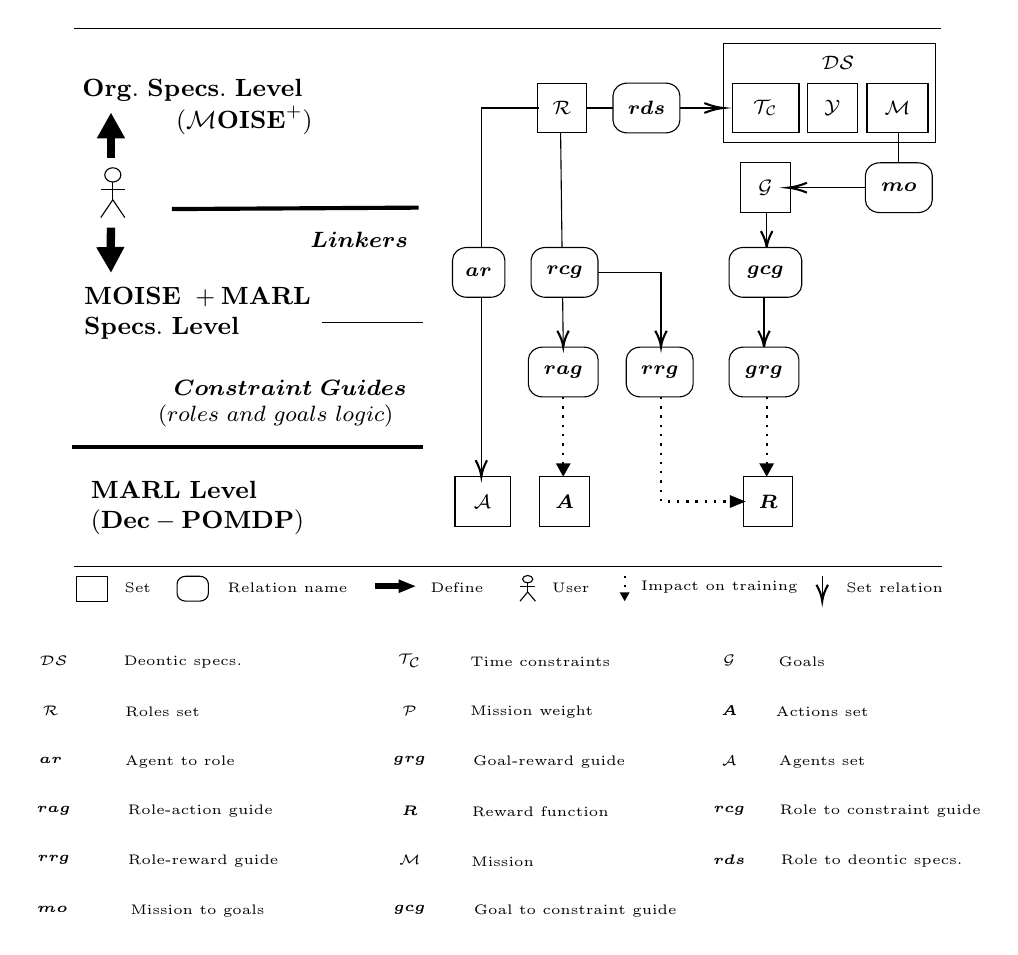
\begin{tikzpicture}[x=0.75pt,y=0.75pt,yscale=-1.2,xscale=1.4]
    %uncomment if require: \path (0,2584); %set diagram left start at 0, and has height of 2584

    %Straight Lines [id:da4973066741986565] 
    \draw [line width=1.5]    (118.21,2302.58) -- (203.1,2302) ;
    %Straight Lines [id:da14807114776731778] 
    \draw    (368.35,2272) -- (368.35,2294) -- (332.16,2294) ;
    \draw [shift={(330.16,2294)}, rotate = 360] [color={rgb, 255:red, 0; green, 0; blue, 0 }  ][line width=0.75]    (6.56,-1.97) .. controls (4.17,-0.84) and (1.99,-0.18) .. (0,0) .. controls (1.99,0.18) and (4.17,0.84) .. (6.56,1.97)   ;
    %Straight Lines [id:da16285043353898754] 
    \draw [line width=1.5]    (83.88,2398) -- (204.61,2398) ;
    %Straight Lines [id:da6299512000169913] 
    \draw    (169.94,2348) -- (204.61,2348) ;
    %Straight Lines [id:da64750232417664] 
    \draw    (84.65,2446) -- (383.15,2446) ;
    %Straight Lines [id:da35895220906699743] 
    \draw    (84.65,2230) -- (383,2230) ;
    %Straight Lines [id:da715014372569708] 
    \draw    (244.68,2262) -- (224.68,2262) -- (224.68,2408) ;
    \draw [shift={(224.68,2410)}, rotate = 270] [color={rgb, 255:red, 0; green, 0; blue, 0 }  ][line width=0.75]    (6.56,-1.97) .. controls (4.17,-0.84) and (1.99,-0.18) .. (0,0) .. controls (1.99,0.18) and (4.17,0.84) .. (6.56,1.97)   ;
    %Straight Lines [id:da71870438525014] 
    \draw    (251.96,2328) -- (286.51,2328) -- (286.51,2356) ;
    \draw [shift={(286.51,2358)}, rotate = 270] [color={rgb, 255:red, 0; green, 0; blue, 0 }  ][line width=0.75]    (6.56,-1.97) .. controls (4.17,-0.84) and (1.99,-0.18) .. (0,0) .. controls (1.99,0.18) and (4.17,0.84) .. (6.56,1.97)   ;
    %Straight Lines [id:da6006267784187092] 
    \draw [line width=0.75]  [dash pattern={on 0.84pt off 2.51pt}]  (252.87,2378) -- (252.87,2407) ;
    \draw [shift={(252.87,2410)}, rotate = 270] [fill={rgb, 255:red, 0; green, 0; blue, 0 }  ][line width=0.08]  [draw opacity=0] (5.36,-2.57) -- (0,0) -- (5.36,2.57) -- cycle    ;
    %Straight Lines [id:da8743336135156266] 
    \draw    (322.88,2304) -- (322.88,2316) ;
    \draw [shift={(322.88,2318)}, rotate = 270] [color={rgb, 255:red, 0; green, 0; blue, 0 }  ][line width=0.75]    (6.56,-1.97) .. controls (4.17,-0.84) and (1.99,-0.18) .. (0,0) .. controls (1.99,0.18) and (4.17,0.84) .. (6.56,1.97)   ;
    %Straight Lines [id:da14641229967966152] 
    \draw [line width=0.75]  [dash pattern={on 0.84pt off 2.51pt}]  (322.88,2378) -- (322.88,2407) ;
    \draw [shift={(322.88,2410)}, rotate = 270] [fill={rgb, 255:red, 0; green, 0; blue, 0 }  ][line width=0.08]  [draw opacity=0] (5.36,-2.57) -- (0,0) -- (5.36,2.57) -- cycle    ;
    %Straight Lines [id:da9260929933425808] 
    \draw [line width=0.75]  [dash pattern={on 0.84pt off 2.51pt}]  (286.51,2378) -- (286.51,2420) -- (312.61,2420) ;
    \draw [shift={(315.61,2420)}, rotate = 180] [fill={rgb, 255:red, 0; green, 0; blue, 0 }  ][line width=0.08]  [draw opacity=0] (5.36,-2.57) -- (0,0) -- (5.36,2.57) -- cycle    ;
    %Straight Lines [id:da3057006030233673] 
    \draw [line width=0.75]  [dash pattern={on 0.84pt off 2.51pt}]  (274,2449.7) -- (274,2457) ;
    \draw [shift={(274,2460)}, rotate = 270] [fill={rgb, 255:red, 0; green, 0; blue, 0 }  ][line width=0.08]  [draw opacity=0] (3.57,-1.72) -- (0,0) -- (3.57,1.72) -- cycle    ;
    %Straight Lines [id:da07288166228322246] 
    \draw    (342,2449.98) -- (342,2458) ;
    \draw [shift={(342,2460)}, rotate = 270] [color={rgb, 255:red, 0; green, 0; blue, 0 }  ][line width=0.75]    (6.56,-1.97) .. controls (4.17,-0.84) and (1.99,-0.18) .. (0,0) .. controls (1.99,0.18) and (4.17,0.84) .. (6.56,1.97)   ;
    %Shape: Ellipse [id:dp8508274348425935] 
    \draw   (95.09,2288.86) .. controls (95.09,2287.28) and (96.33,2286) .. (97.85,2286) .. controls (99.38,2286) and (100.62,2287.28) .. (100.62,2288.86) .. controls (100.62,2290.44) and (99.38,2291.71) .. (97.85,2291.71) .. controls (96.33,2291.71) and (95.09,2290.44) .. (95.09,2288.86) -- cycle ;
    %Straight Lines [id:da3825450168053828] 
    \draw    (97.85,2291.71) -- (97.85,2298.86) ;
    %Straight Lines [id:da521321206042058] 
    \draw    (97.85,2298.86) -- (93.71,2306) ;
    %Straight Lines [id:da055514206493922025] 
    \draw    (97.85,2298.86) -- (102,2306) ;
    %Straight Lines [id:da8996496708356774] 
    \draw    (102,2294.57) -- (93.71,2294.57) ;

    %Straight Lines [id:da31678488015771755] 
    \draw [line width=2.25]    (188,2454) -- (196.97,2454) ;
    \draw [shift={(201.97,2454)}, rotate = 180] [fill={rgb, 255:red, 0; green, 0; blue, 0 }  ][line width=0.08]  [draw opacity=0] (5.72,-2.75) -- (0,0) -- (5.72,2.75) -- cycle    ;
    %Shape: Ellipse [id:dp3927356466672782] 
    \draw   (238.88,2451.17) .. controls (238.88,2450.36) and (239.67,2449.7) .. (240.64,2449.7) .. controls (241.61,2449.7) and (242.4,2450.36) .. (242.4,2451.17) .. controls (242.4,2451.99) and (241.61,2452.65) .. (240.64,2452.65) .. controls (239.67,2452.65) and (238.88,2451.99) .. (238.88,2451.17) -- cycle ;
    %Straight Lines [id:da3365602555559104] 
    \draw    (240.64,2452.65) -- (240.64,2456.32) ;
    %Straight Lines [id:da7990875235744026] 
    \draw    (240.64,2456.32) -- (238,2460) ;
    %Straight Lines [id:da23945649338821617] 
    \draw    (240.64,2456.32) -- (243.28,2460) ;
    %Straight Lines [id:da11927353559661591] 
    \draw    (243.28,2454.12) -- (238,2454.12) ;

    %Straight Lines [id:da5816423191130675] 
    \draw    (251.96,2272) -- (252.85,2356) ;
    \draw [shift={(252.87,2358)}, rotate = 269.39] [color={rgb, 255:red, 0; green, 0; blue, 0 }  ][line width=0.75]    (6.56,-1.97) .. controls (4.17,-0.84) and (1.99,-0.18) .. (0,0) .. controls (1.99,0.18) and (4.17,0.84) .. (6.56,1.97)   ;
    %Straight Lines [id:da9310455126832857] 
    \draw    (321.97,2338) -- (321.97,2356) ;
    \draw [shift={(321.97,2358)}, rotate = 270] [color={rgb, 255:red, 0; green, 0; blue, 0 }  ][line width=0.75]    (6.56,-1.97) .. controls (4.17,-0.84) and (1.99,-0.18) .. (0,0) .. controls (1.99,0.18) and (4.17,0.84) .. (6.56,1.97)   ;
    %Shape: Rectangle [id:dp293492578719597] 
    \draw   (120,2453) .. controls (120,2451.34) and (121.34,2450) .. (123,2450) -- (127.72,2450) .. controls (129.37,2450) and (130.72,2451.34) .. (130.72,2453) -- (130.72,2457) .. controls (130.72,2458.66) and (129.37,2460) .. (127.72,2460) -- (123,2460) .. controls (121.34,2460) and (120,2458.66) .. (120,2457) -- cycle ;
    %Straight Lines [id:da33566712615128225] 
    \draw    (261.05,2262) -- (306,2262) ;
    \draw [shift={(308,2262)}, rotate = 180] [color={rgb, 255:red, 0; green, 0; blue, 0 }  ][line width=0.75]    (6.56,-1.97) .. controls (4.17,-0.84) and (1.99,-0.18) .. (0,0) .. controls (1.99,0.18) and (4.17,0.84) .. (6.56,1.97)   ;
    %Shape: Rectangle [id:dp28383270948937667] 
    \draw   (308,2236) -- (381.08,2236) -- (381.08,2276) -- (308,2276) -- cycle ;
    %Straight Lines [id:da18020989903965012] 
    \draw [line width=3]    (97.22,2282) -- (97.22,2270) ;
    \draw [shift={(97.22,2264)}, rotate = 90] [fill={rgb, 255:red, 0; green, 0; blue, 0 }  ][line width=0.08]  [draw opacity=0] (10.18,-4.89) -- (0,0) -- (10.18,4.89) -- cycle    ;
    %Straight Lines [id:da018421338049046554] 
    \draw [line width=3]    (97.22,2310) -- (97.11,2322.37) ;
    \draw [shift={(97.22,2328)}, rotate = 268.86] [fill={rgb, 255:red, 0; green, 0; blue, 0 }  ][line width=0.08]  [draw opacity=0] (10.18,-4.89) -- (0,0) -- (10.18,4.89) -- cycle    ;
    %Shape: Rectangle [id:dp7281037051878541] 
    \draw   (85.42,2450) -- (96.13,2450) -- (96.13,2460) -- (85.42,2460) -- cycle ;

    % Text Node
    \draw (362,2544.5) node  [font=\tiny] [align=left] {Role to constraint guide};
    % Text Node
    \draw (342,2524.5) node  [font=\tiny] [align=left] {Agents set};
    % Text Node
    \draw (342,2504.5) node  [font=\tiny] [align=left] {Actions set};
    % Text Node
    \draw (257,2584.5) node  [font=\tiny] [align=left] {Goal to constraint guide};
    % Text Node
    \draw (335,2484.5) node  [font=\tiny] [align=left] {Goals};
    % Text Node
    \draw (359,2564.5) node  [font=\tiny] [align=left] {Role to deontic specs.};
    % Text Node
    \draw (232,2564.5) node  [font=\tiny] [align=left] {Mission};
    % Text Node
    \draw (245,2544.5) node  [font=\tiny] [align=left] {Reward function};
    % Text Node
    \draw (248,2524.5) node  [font=\tiny] [align=left] {Goal-reward guide};
    % Text Node
    \draw (242,2504.5) node  [font=\tiny] [align=left] {Mission weight};
    % Text Node
    \draw (245,2484.5) node  [font=\tiny] [align=left] {Time constraints};
    % Text Node
    \draw (127,2584.5) node  [font=\tiny] [align=left] {Mission to goals};
    % Text Node
    \draw (129,2564.5) node  [font=\tiny] [align=left] {Role-reward guide};
    % Text Node
    \draw (128,2544.5) node  [font=\tiny] [align=left] {Role-action guide};
    % Text Node
    \draw (121,2524.5) node  [font=\tiny] [align=left] {Agent to role};
    % Text Node
    \draw (115,2504.5) node  [font=\tiny] [align=left] {Roles set};
    % Text Node
    \draw (122,2484.5) node  [font=\tiny] [align=left] {Deontic specs.};
    % Text Node
    \draw (310,2544) node  [font=\tiny] [align=left] {$\displaystyle \boldsymbol{rcg}$};
    % Text Node
    \draw (200,2504) node  [font=\tiny] [align=left] {$\displaystyle \mathcal{P}$};
    % Text Node
    \draw (200,2484) node  [font=\tiny] [align=left] {$\displaystyle \mathcal{T_{C}}$};
    % Text Node
    \draw (200,2564) node  [font=\tiny] [align=left] {$\displaystyle \mathcal{M}$};
    % Text Node
    \draw (77.5,2484) node  [font=\tiny] [align=left] {$\displaystyle \mathcal{DS}$};
    % Text Node
    \draw (310,2564) node  [font=\tiny] [align=left] {$\displaystyle \boldsymbol{rds}$};
    % Text Node
    \draw (310,2504) node  [font=\tiny] [align=left] {$\displaystyle \boldsymbol{A}$};
    % Text Node
    \draw (200,2544) node  [font=\tiny] [align=left] {$\displaystyle \boldsymbol{R}$};
    % Text Node
    \draw (310,2524) node  [font=\tiny] [align=left] {$\displaystyle \mathcal{A}$};
    % Text Node
    \draw (200,2524) node  [font=\tiny] [align=left] {$\displaystyle \boldsymbol{grg}$};
    % Text Node
    \draw (77.5,2564) node  [font=\tiny] [align=left] {$\displaystyle \boldsymbol{rrg}$};
    % Text Node
    \draw (77.5,2544) node  [font=\tiny] [align=left] {$\displaystyle \boldsymbol{rag}$};
    % Text Node
    \draw (200,2584) node  [font=\tiny] [align=left] {$\displaystyle \boldsymbol{gcg}$};
    % Text Node
    \draw (76.5,2524) node  [font=\tiny] [align=left] {$\displaystyle \boldsymbol{ar}$};
    % Text Node
    \draw (77,2584) node  [font=\tiny] [align=left] {$\displaystyle \boldsymbol{mo}$};
    % Text Node
    \draw (76.5,2504) node  [font=\tiny] [align=left] {$\displaystyle \mathcal{R}$};
    % Text Node
    \draw (310,2484) node  [font=\tiny] [align=left] {$\displaystyle \mathcal{G}$};


    % Text Node
    \draw  [fill={rgb, 255:red, 255; green, 255; blue, 255 }  ,fill opacity=1 ]  (241.82,2323) .. controls (241.82,2320.24) and (244.06,2318) .. (246.82,2318) -- (259.82,2318) .. controls (262.58,2318) and (264.82,2320.24) .. (264.82,2323) -- (264.82,2333) .. controls (264.82,2335.76) and (262.58,2338) .. (259.82,2338) -- (246.82,2338) .. controls (244.06,2338) and (241.82,2335.76) .. (241.82,2333) -- cycle  ;
    \draw (253.32,2328) node  [font=\scriptsize] [align=left] {$\displaystyle \boldsymbol{rcg}$};
    % Text Node
    \draw    (337,2252) -- (354,2252) -- (354,2272) -- (337,2272) -- cycle  ;
    \draw (345.5,2262) node  [font=\scriptsize] [align=left] {$\displaystyle \mathcal{Y}$};
    % Text Node
    \draw    (311,2252) -- (334,2252) -- (334,2272) -- (311,2272) -- cycle  ;
    \draw (322.5,2262) node  [font=\scriptsize] [align=left] {$\displaystyle \mathcal{T_{C}}$};
    % Text Node
    \draw    (357.39,2252) -- (378.39,2252) -- (378.39,2272) -- (357.39,2272) -- cycle  ;
    \draw (367.89,2262) node  [font=\scriptsize] [align=left] {$\displaystyle \mathcal{M}$};
    % Text Node
    \draw (347.43,2244) node  [font=\scriptsize] [align=left] {$\displaystyle \mathcal{DS}$};
    % Text Node
    \draw  [fill={rgb, 255:red, 255; green, 255; blue, 255 }  ,fill opacity=1 ]  (270,2257) .. controls (270,2254.24) and (272.24,2252) .. (275,2252) -- (288,2252) .. controls (290.76,2252) and (293,2254.24) .. (293,2257) -- (293,2267) .. controls (293,2269.76) and (290.76,2272) .. (288,2272) -- (275,2272) .. controls (272.24,2272) and (270,2269.76) .. (270,2267) -- cycle  ;
    \draw (281.5,2262) node  [font=\scriptsize] [align=left] {$\displaystyle \boldsymbol{rds}$};
    % Text Node
    \draw (158,2454.5) node  [font=\tiny] [align=left] {Relation name};
    % Text Node
    \draw (106.46,2454.5) node  [font=\tiny] [align=left] {Set};
    % Text Node
    \draw (255.47,2454.5) node  [font=\tiny] [align=left] {User};
    % Text Node
    \draw (216.32,2454.5) node  [font=\tiny] [align=left] {Define};
    % Text Node
    \draw (366.91,2454.5) node  [font=\tiny] [align=left] {Set relation};
    % Text Node
    \draw (306.61,2454.5) node  [font=\tiny] [align=left] {Impact on training};
    % Text Node
    \draw    (244.82,2410) -- (261.82,2410) -- (261.82,2430) -- (244.82,2430) -- cycle  ;
    \draw (253.32,2420) node  [font=\scriptsize] [align=left] {$\displaystyle \boldsymbol{A}$};
    % Text Node
    \draw    (314.84,2410) -- (331.84,2410) -- (331.84,2430) -- (314.84,2430) -- cycle  ;
    \draw (323.34,2420) node  [font=\scriptsize] [align=left] {$\displaystyle \boldsymbol{R}$};
    % Text Node
    \draw    (215.63,2410) -- (234.63,2410) -- (234.63,2430) -- (215.63,2430) -- cycle  ;
    \draw (225.13,2420) node  [font=\scriptsize] [align=left] {$\displaystyle \mathcal{A}$};
    % Text Node
    \draw  [fill={rgb, 255:red, 255; green, 255; blue, 255 }  ,fill opacity=1 ]  (309.97,2363) .. controls (309.97,2360.24) and (312.21,2358) .. (314.97,2358) -- (328.97,2358) .. controls (331.73,2358) and (333.97,2360.24) .. (333.97,2363) -- (333.97,2373) .. controls (333.97,2375.76) and (331.73,2378) .. (328.97,2378) -- (314.97,2378) .. controls (312.21,2378) and (309.97,2375.76) .. (309.97,2373) -- cycle  ;
    \draw (321.97,2368) node  [font=\scriptsize] [align=left] {$\displaystyle \boldsymbol{grg}$};
    % Text Node
    \draw    (274.56,2363) .. controls (274.56,2360.24) and (276.8,2358) .. (279.56,2358) -- (292.56,2358) .. controls (295.32,2358) and (297.56,2360.24) .. (297.56,2363) -- (297.56,2373) .. controls (297.56,2375.76) and (295.32,2378) .. (292.56,2378) -- (279.56,2378) .. controls (276.8,2378) and (274.56,2375.76) .. (274.56,2373) -- cycle  ;
    \draw (286.06,2368) node  [font=\scriptsize] [align=left] {$\displaystyle \boldsymbol{rrg}$};
    % Text Node
    \draw    (240.87,2363) .. controls (240.87,2360.24) and (243.11,2358) .. (245.87,2358) -- (259.87,2358) .. controls (262.63,2358) and (264.87,2360.24) .. (264.87,2363) -- (264.87,2373) .. controls (264.87,2375.76) and (262.63,2378) .. (259.87,2378) -- (245.87,2378) .. controls (243.11,2378) and (240.87,2375.76) .. (240.87,2373) -- cycle  ;
    \draw (252.87,2368) node  [font=\scriptsize] [align=left] {$\displaystyle \boldsymbol{rag}$};
    % Text Node
    \draw (156.15,2380.5) node  [font=\footnotesize] [align=left] {$\displaystyle  \begin{array}{{>{\displaystyle}l}}
                \ \ \boldsymbol{Constraint\ Guides} \\
                ( roles\ and\ goals\ logic)
            \end{array}$};
    % Text Node
    \draw  [fill={rgb, 255:red, 255; green, 255; blue, 255 }  ,fill opacity=1 ]  (309.93,2323) .. controls (309.93,2320.24) and (312.17,2318) .. (314.93,2318) -- (329.93,2318) .. controls (332.69,2318) and (334.93,2320.24) .. (334.93,2323) -- (334.93,2333) .. controls (334.93,2335.76) and (332.69,2338) .. (329.93,2338) -- (314.93,2338) .. controls (312.17,2338) and (309.93,2335.76) .. (309.93,2333) -- cycle  ;
    \draw (322.43,2328) node  [font=\scriptsize] [align=left] {$\displaystyle \boldsymbol{gcg}$};
    % Text Node
    \draw  [fill={rgb, 255:red, 255; green, 255; blue, 255 }  ,fill opacity=1 ]  (214.77,2323) .. controls (214.77,2320.24) and (217.01,2318) .. (219.77,2318) -- (227.77,2318) .. controls (230.53,2318) and (232.77,2320.24) .. (232.77,2323) -- (232.77,2333) .. controls (232.77,2335.76) and (230.53,2338) .. (227.77,2338) -- (219.77,2338) .. controls (217.01,2338) and (214.77,2335.76) .. (214.77,2333) -- cycle  ;
    \draw (223.77,2328) node  [font=\scriptsize] [align=left] {$\displaystyle \boldsymbol{ar}$};
    % Text Node
    \draw  [fill={rgb, 255:red, 255; green, 255; blue, 255 }  ,fill opacity=1 ]  (356.85,2289) .. controls (356.85,2286.24) and (359.08,2284) .. (361.85,2284) -- (374.85,2284) .. controls (377.61,2284) and (379.85,2286.24) .. (379.85,2289) -- (379.85,2299) .. controls (379.85,2301.76) and (377.61,2304) .. (374.85,2304) -- (361.85,2304) .. controls (359.08,2304) and (356.85,2301.76) .. (356.85,2299) -- cycle  ;
    \draw (368.35,2294) node  [font=\scriptsize] [align=left] {$\displaystyle \boldsymbol{mo}$};
    % Text Node
    \draw (127,2344.5) node  [font=\small] [align=left] {$\displaystyle  \begin{array}{{>{\displaystyle}l}}
                \mathbf{MOISE\ +MARL} \\
                \mathbf{Specs.\ Level}
            \end{array}$};
    % Text Node
    \draw (127,2422.5) node  [font=\small] [align=left] {$\displaystyle  \begin{array}{{>{\displaystyle}l}}
                \mathbf{MARL\ Level} \\
                \mathbf{(Dec-POMDP)}
            \end{array}$};
    % Text Node
    \draw    (243.91,2252) -- (260.91,2252) -- (260.91,2272) -- (243.91,2272) -- cycle  ;
    \draw (252.41,2262) node  [font=\scriptsize] [align=left] {$\displaystyle \mathcal{R}$};
    % Text Node
    \draw (182.64,2315) node  [font=\footnotesize] [align=left] {$\displaystyle \boldsymbol{Linkers}$};
    % Text Node
    \draw    (313.93,2284) -- (330.93,2284) -- (330.93,2304) -- (313.93,2304) -- cycle  ;
    \draw (322.43,2294) node  [font=\scriptsize] [align=left] {$\displaystyle \mathcal{G}$};
    % Text Node
    \draw (127,2261.5) node  [font=\small] [align=left] {$\displaystyle  \begin{array}{{>{\displaystyle}l}}
                \mathbf{{\displaystyle Org.\ Specs.\ Level}} \\
                {\displaystyle \ \ \ \ \ \ \ \ \ \ \ (\mathcal{M}\mathbf{OISE^+})}
            \end{array}$};


\end{tikzpicture}
    \caption{A minimal view of the MOISE+MARL framework:
        Users first define $\mathcal{M}OISE^+$ specifications, which include roles ($\mathcal{R}$) and missions ($\mathcal{M}$), both associated through $rds$. They then create MOISE+MARL specifications by first defining \textbf{Constraint guides} such as $rag$ and $rrg$ to specify role logic, and $grg$ for goal logic. 
        Next, \textbf{Linkers} are used to connect agents with roles through $ar$ and to link the logic of the constraint guides to the defined $\mathcal{M}OISE^+$ specifications. Once this is set up, roles can be assigned to agents, and the MARL framework updates accordingly during training.
    }
    \label{fig:mm_synthesis}
\end{figure}

\noindent MOISE+MARL introduces means to control or guide the agents' training in MARL. Its core contribution ar the \textbf{Constraint Guides}, which are three new relations introduced to describe the logics of roles and goals in the Dec-POMDP formalism:
%
\begin{itemize}
    % \begin{enumerate*}[label={\roman*) },itemjoin={; \quad}]
    
    \item \textbf{Role Action Guide} \quad $rag: H \times \Omega \rightarrow \mathcal{P}(A \times \mathbb{R})$, the relation that models a role as a set of rules which, for each pair consisting of a history $h \in H$ and an observation received by the agent $\omega \in \Omega$, associates expected actions $A \in \mathcal{P}(A)$ each associated with a constraint hardness $ch \in [0,1]$ ($ch = 1$ by default). By restricting the choice of the next action among those authorized, the agent is forced to adhere to the role's expected behavior
    \item \textbf{Role Reward Guide} \quad $rrg: H \times \Omega \times A \to \mathbb{R} = \{r_m \text{ if } a \notin A_\omega \text{, } rag(h, \omega) \allowbreak = \allowbreak A_\omega \times \mathbb{R} \text{, } h \in H; \text{ else } 0\}$, the relation that models a role by adding a penalty $r_m$ to the global reward if the last action chosen by the agent $a \in A$ is not authorized. This is intended to encourage the agent to adhere to the expected behavior
    \item \textbf{Goal Reward Guide} \quad $grg: H \rightarrow \mathbb{R}$, the relation that models a goal as a soft constraint adding a reward bonus $r_b \in \mathbb{R}$ if the agent's history $h \in H$ contains a goal's characteristic sub-sequence $h_g \in H_g$, encouraging the agent to reach it.
          % \end{enumerate*}
\end{itemize}

\noindent Finally, we introduce the \textbf{Linkers} to link the $\mathcal{M}OISE^+$ organizational specifications with constraint guides and agents:
%
\begin{itemize}
    % \begin{enumerate*}[label={\roman*) },itemjoin={; \quad}]
    
    \item \textbf{Agent to Role} \quad $ar: \mathcal{A} \to \mathcal{R}$, the bijective relation linking an agent to a role;
    \item \textbf{Role to Constraint Guide} \quad $rcg: \mathcal{R} \rightarrow rag \cup rrg$, the relation associating each $\mathcal{M}OISE^+$ role to a $rag$ or $rrg$ relation, forcing/encouraging the agent to follow the expected actions for the role $\rho \in \mathcal{R}$;
    \item \textbf{Goal to Constraint Guide} \quad $gcg: \mathcal{G} \rightarrow grg$, the relation linking goals to $grg$ relations, representing goals as rewards in MARL.
          % \end{enumerate*}
\end{itemize}

\paragraph{\textbf{Resolving the Dec-POMDP with MOISE+MARL}}

A MOISE+MARL model is defined as $\mathcal{MM} = \langle \mathcal{OS}, ar, rcg, gcg, rag, rrg, grg \rangle$.
Solving a Dec-POMDP with $mm \in \mathcal{MM}$ consists in finding a joint policy $\pi^j = {\pi^j_0, \pi^j_1, \dots, \pi^j_n}$ that maximizes the expected cumulative reward (or satisfies a minimal threshold), represented by the state-value function $V^{\pi^j}$. This value reflects the return from an initial state $s \in S$ when applying successive joint actions $a^j \in A^n$ under the additional organizational constraints.
%
The definition of $V^{\pi^j}$ follows the sequential and cyclic agent execution scheme (AEC mode), and is formalized in \hyperref[eq:single_value_function]{Definition 1}, incorporating role-based (in red) and mission-based (in blue) adaptations that influence both the action space and the reward.
\autoref{fig:mm_synthesis} illustrates how the MOISE+ specifications are integrated into the Dec-POMDP resolution via the MOISE+MARL framework.


\begin{figure*}[h!]
    \label{eq:single_value_function}
    \raggedright
    \textbf{\textit{Definition 1} \quad State-Value function adapted to constraint guides in AEC:}
    
    \begin{scriptsize}
        \vspace{-0.6cm}
        \begin{gather*}
            V^{\pi^j}(s_t) = \hspace{-0.75cm}
            %
            \sum_{\textcolor{red}{ \substack{a_{t} \in A \text{ if } rn() < ch_{t}, \\
                        a_{t} \in A_{t} \text{ else}}
                }}{\hspace{-0.7cm} \pi_i(a_{t} | \omega_t)}
            %
            \sum_{s_{t+1} \in S}
            %
            {\hspace{-0.1cm} T(s_{t+1} | s_t, a_{t})
            \Bigl[R(s_t,a_{t},s_{t+1}) + \hspace{-0.1cm}
            \textcolor{blue}{ \sum_{m \in \mathcal{M}_i}{ \hspace{-0.1cm} v_m(t) \frac{grg_m(h_{t+1})}{1 - p + \epsilon} } }
            + } \\
            {\textcolor{red}{(1-ch_t) \times rrg(\omega_t,a_{t+1})} + V^{\pi^j_{i+1 \ mod \ n}}(s_{t+1})\Bigr]}
        \end{gather*}
        %
        \vspace{-0.5cm}
        \textcolor{red}{\[\text{ \hspace{-0.1cm} With } rag(h_t, \omega_t) = A_{t} \times \mathbb{R} \text{, } \langle a_t, ch_{t} \rangle \in A_{t} \times \mathbb{R} \text{ ; } rn: \emptyset \to [0,1[ \text{, a uniform random function}\]}
        %
        \vspace{-0.6cm}
        \textcolor{blue}{
            \begin{gather*}
                \hspace{-0.001cm}
                \text{With } \omega_t = O(\omega_t | s_t, a_t) \text{ ; } h_t = \{h_0 = \langle \rangle, h_{t+1} = \langle h_t, \langle \omega_{t+1}, a_{t+1} \rangle \rangle \} \text{ ; } \epsilon \in \mathbb{R}_{>0} \text{ ; } grg_m(h) = 
            \end{gather*}
        }
        \vspace{-0.95cm}
        \textcolor{blue}{
            \begin{gather*}
                \hspace{-0.5cm} \sum_{\hspace{0.3cm}(grg_i,w_i) \in mo(m)}{\hspace{-0.9cm} w_i \times grg_i(h)}
                \text{ ; } v_m(t) = \{ 1 \text{ if } t \in t_c \text{ ; else } 0 \} \text{ ; } \mathcal{M}_i = \{m_j | \langle ar(i),m_j,t_c,p \rangle \in \mathcal{M}\}
            \end{gather*}
        }
        \vspace{-0.6cm}
    \end{scriptsize}
    
\end{figure*}

\noindent At each time step $t \in \mathbb{N}$ (starting from $t=0$), agent $i = t \bmod n$ is assigned to role $\rho_i = ar(i)$. For each temporally valid deontic specification $d_i = rds(\rho_i) = \langle tc_i, y_i, m_i \rangle$, the agent is permitted ($y_i = 0$) or obligated ($y_i = 1$) to commit to mission $m_i \in \mathcal{M}$, with goal set $\mathcal{G}_{m_i} = mo(m_i)$ and $n \in \mathbb{N}$ agents.
%
Upon observing $\omega_t$, the agent selects an action from $A_t$ (the role-expected actions) with probability $ch_t$, or from $A$ otherwise. If $ch_t = 1$, the agent is strictly constrained by its role.
%
The selected action transitions the system from $s_t$ to $s_{t+1}$, yields observation $\omega_{t+1}$, and returns a reward composed of:
i) bonuses for achieved goals in valid missions (via Goal Reward Guides), weighted by $\frac{1}{1 - p + \epsilon}$;
ii) penalties from the Role Reward Guide, scaled by $ch_t$.
%
The process continues in state $s_{t+1}$ with agent $(i + 1) \bmod n$.

\subsection{The TEMM method}
\label{sec:TEMM_algorithm}

The TEMM method is part of the explanation component of the MOISE+MARL framework. It leverages unsupervised learning techniques to infer organizational specifications from observed agent trajectories. It allows computing the organizational fit between emergent behaviors and expected roles, goals, and missions.

\textbf{1) Roles and role inheritance.} \quad TEMM defines a role $\rho$ as a policy whose agents share a \textit{Common Longest Sequence} (CLS) in their histories. A role $\rho_2$ inherits from $\rho_1$ if $\text{CLS}(\rho_2) \subseteq \text{CLS}(\rho_1)$. Hierarchical clustering is used to extract these CLSs and role hierarchies from trajectories. The \textbf{structural organizational fit} is computed as the distance between actual agent behaviors and inferred role sequences.

\textbf{2) Goals, plans, and missions.} \quad Goals are identified as clusters of joint-observations commonly reached in successful trajectories, using K-means over trajectory embeddings. Plans are inferred as sub-sequences of transitions that consistently lead to goals. A \textbf{mission} groups goals pursued collectively by one or more agents. The \textbf{functional organizational fit} quantifies how well current behaviors match inferred goals and missions.

\textbf{3) Permissions and obligations.} \quad Permissions and obligations are derived by examining whether agents fulfilling a role consistently (or exclusively) achieve certain missions under time constraints. Obligations imply exclusivity, whereas permissions imply optionality. The global \textbf{organizational fit} is obtained by aggregating structural and functional scores.

While clustering hyperparameters may require manual tuning to ensure robust role and goal extraction, TEMM offers a principled way to analyze emergent organizational behaviors and refine specifications accordingly.



\subsection{Learning World Models}

In Reinforcement Learning (RL), particularly under partial observability, \textbf{World Models}~\cite{ha2018recurrent, hafner2020dream} aim to learn internal models approximating both the environment's transition and observation dynamics. Such models enable agents to perform planning, improve sample efficiency, and facilitate safe exploration. This modeling approach belongs to the \textit{model-based RL} (MBRL) paradigm~\cite{moerland2020model}, and is especially useful for automatically constructing high-fidelity simulation models even when explicit environment representations are unavailable.

Formally, at each time step $t$, let $\omega_t \in \Omega$ denote the current high-dimensional observation, $a_t \in A$ the action taken, and $\tilde{h}_{t-1} \in \mathcal{H}$ the recurrent hidden state summarizing the interaction history up to $t-1$. Since observations are typically high-dimensional (e.g., images, complex state vectors), an encoder $Enc: \Omega \rightarrow Z$ is first applied to project observations into a compact latent space $Z$ with $z_t = Enc(\omega_t)$, where $\dim(Z) \ll \dim(\Omega)$.

The core temporal structure is modeled using a \textbf{Recurrent Latent Dynamics Model (RLDM)}~\cite{hafner2020dream} $\mathcal{T}^{z} = f(g(h_{t-1},z_t, a_t))$, which predicts the next latent state $z_{t+1}$ by updating the recurrent hidden state with $f$ and applying latent dynamics with $g$:
$h_t = f(h_{t-1}, z_t, a_t), z_{t+1} = g(h_t)$
where $f(\cdot)$ typically corresponds to a recurrent neural network (e.g., LSTM~\cite{hochreiter1997long}) applied to the concatenation of $h_{t-1}$, $z_t$, and $a_t$, and $g(\cdot)$ maps the recurrent state to the next observation latent representation (often implmented as an MLP~\cite{hochreiter1997long}).

The predicted latent state is then decoded via $Dec: Z \rightarrow \Omega$ into the predicted observation $\hat{\omega}_{t+1} = Dec(z_{t+1})$. The entire model is jointly trained to minimize both the \emph{reconstruction loss} $\|\omega_{t+1} - \hat{\omega}_{t+1}\|$ in observation space, and optionally, a \emph{latent prediction loss} to stabilize latent dynamics learning.

The recurrent hidden state $\tilde{h}_t$ serves as a compact summary of the full interaction history up to time $t$, avoiding the need to explicitly store long observation-action trajectories.
For simplicity of notation, we define the full composition that directly maps current observation, action, and recurrent state to the next predicted observation as the \textbf{Observation Prediction Model}:
\[
    \mathcal{T}(h_{t-1}, \omega_t, a_t) := Dec(g(f(h_{t-1}, Enc(\omega_t), a_t))) = \hat{\omega}_{t+1}.
\]



\section{The MAMAD method}\label{sec:mamad}

\subsection{General overview of the method}

The MAMAD~\footnotemark[1] method is built around four main activities: (1) modeling the environment, goal, and organizational constraints, (2) learning policies using various MARL algorithms, (3) analyzing behaviors and inferring organizational specifications with a proposed method, and (4) maintaining consistency between the simulated and real environments by deploying trained policies and updating the simulation. This approach guides the agent learning process while enforcing strict organizational constraints, ensuring the efficiency of the learned policies. The lifecycle of a MAMAD-designed MAS is illustrated in \autoref{fig:cycle}.
%
\begin{figure}[h!]
    \centering
    


\tikzset{every picture/.style={line width=0.75pt}} %set default line width to 0.75pt        

\begin{tikzpicture}[x=0.75pt,y=0.75pt,yscale=-1,xscale=1]
%uncomment if require: \path (0,3307); %set diagram left start at 0, and has height of 3307

%Shape: Smiley Face [id:dp29065495216725257] 
\draw  [line width=1.5]  (85.38,2800.11) .. controls (85.38,2797.7) and (87.16,2795.75) .. (89.36,2795.75) .. controls (91.55,2795.75) and (93.34,2797.7) .. (93.34,2800.11) .. controls (93.34,2802.52) and (91.55,2804.48) .. (89.36,2804.48) .. controls (87.16,2804.48) and (85.38,2802.52) .. (85.38,2800.11) -- cycle ; \draw  [line width=1.5]  (87.61,2798.63) .. controls (87.61,2798.39) and (87.78,2798.19) .. (88,2798.19) .. controls (88.22,2798.19) and (88.4,2798.39) .. (88.4,2798.63) .. controls (88.4,2798.87) and (88.22,2799.07) .. (88,2799.07) .. controls (87.78,2799.07) and (87.61,2798.87) .. (87.61,2798.63) -- cycle ; \draw  [line width=1.5]  (90.31,2798.63) .. controls (90.31,2798.39) and (90.49,2798.19) .. (90.71,2798.19) .. controls (90.93,2798.19) and (91.11,2798.39) .. (91.11,2798.63) .. controls (91.11,2798.87) and (90.93,2799.07) .. (90.71,2799.07) .. controls (90.49,2799.07) and (90.31,2798.87) .. (90.31,2798.63) -- cycle ; \draw  [line width=1.5]  (87.37,2801.86) .. controls (88.69,2803.02) and (90.02,2803.02) .. (91.35,2801.86) ;
%Shape: Rectangle [id:dp42672371521059915] 
\draw  [dash pattern={on 5.63pt off 4.5pt}][line width=1.5]  (74.03,2763.75) -- (192,2763.75) -- (192,2813.93) -- (74.03,2813.93) -- cycle ;
%Shape: Smiley Face [id:dp9817389082285293] 
\draw  [line width=1.5]  (144.45,2803.6) .. controls (144.45,2801.19) and (146.24,2799.24) .. (148.43,2799.24) .. controls (150.63,2799.24) and (152.41,2801.19) .. (152.41,2803.6) .. controls (152.41,2806.01) and (150.63,2807.97) .. (148.43,2807.97) .. controls (146.24,2807.97) and (144.45,2806.01) .. (144.45,2803.6) -- cycle ; \draw  [line width=1.5]  (146.68,2802.12) .. controls (146.68,2801.88) and (146.86,2801.68) .. (147.08,2801.68) .. controls (147.3,2801.68) and (147.48,2801.88) .. (147.48,2802.12) .. controls (147.48,2802.36) and (147.3,2802.56) .. (147.08,2802.56) .. controls (146.86,2802.56) and (146.68,2802.36) .. (146.68,2802.12) -- cycle ; \draw  [line width=1.5]  (149.39,2802.12) .. controls (149.39,2801.88) and (149.57,2801.68) .. (149.79,2801.68) .. controls (150.01,2801.68) and (150.18,2801.88) .. (150.18,2802.12) .. controls (150.18,2802.36) and (150.01,2802.56) .. (149.79,2802.56) .. controls (149.57,2802.56) and (149.39,2802.36) .. (149.39,2802.12) -- cycle ; \draw  [line width=1.5]  (146.44,2805.35) .. controls (147.77,2806.51) and (149.1,2806.51) .. (150.42,2805.35) ;
%Shape: Smiley Face [id:dp49419175504212776] 
\draw  [line width=1.5]  (179.09,2781.5) .. controls (179.09,2779.09) and (180.87,2777.13) .. (183.06,2777.13) .. controls (185.26,2777.13) and (187.04,2779.09) .. (187.04,2781.5) .. controls (187.04,2783.91) and (185.26,2785.86) .. (183.06,2785.86) .. controls (180.87,2785.86) and (179.09,2783.91) .. (179.09,2781.5) -- cycle ; \draw  [line width=1.5]  (181.31,2780.01) .. controls (181.31,2779.77) and (181.49,2779.58) .. (181.71,2779.58) .. controls (181.93,2779.58) and (182.11,2779.77) .. (182.11,2780.01) .. controls (182.11,2780.25) and (181.93,2780.45) .. (181.71,2780.45) .. controls (181.49,2780.45) and (181.31,2780.25) .. (181.31,2780.01) -- cycle ; \draw  [line width=1.5]  (184.02,2780.01) .. controls (184.02,2779.77) and (184.2,2779.58) .. (184.42,2779.58) .. controls (184.64,2779.58) and (184.81,2779.77) .. (184.81,2780.01) .. controls (184.81,2780.25) and (184.64,2780.45) .. (184.42,2780.45) .. controls (184.2,2780.45) and (184.02,2780.25) .. (184.02,2780.01) -- cycle ; \draw  [line width=1.5]  (181.07,2783.24) .. controls (182.4,2784.4) and (183.73,2784.4) .. (185.05,2783.24) ;
%Flowchart: Punched Tape [id:dp3565745198144521] 
\draw  [fill={rgb, 255:red, 255; green, 255; blue, 255 }  ,fill opacity=1 ] (291.67,2877.34) .. controls (291.67,2880.23) and (301.36,2882.58) .. (313.31,2882.58) .. controls (325.26,2882.58) and (334.95,2880.23) .. (334.95,2877.34) .. controls (334.95,2874.45) and (344.64,2872.11) .. (356.6,2872.11) .. controls (368.55,2872.11) and (378.24,2874.45) .. (378.24,2877.34) -- (378.24,2919.23) .. controls (378.24,2916.34) and (368.55,2913.99) .. (356.6,2913.99) .. controls (344.64,2913.99) and (334.95,2916.34) .. (334.95,2919.23) .. controls (334.95,2922.12) and (325.26,2924.46) .. (313.31,2924.46) .. controls (301.36,2924.46) and (291.67,2922.12) .. (291.67,2919.23) -- cycle ;
%Straight Lines [id:da23451091058783402] 
\draw [line width=1.5]    (320.63,2891.89) -- (349.47,2889.91) ;
\draw [shift={(352.46,2889.7)}, rotate = 176.08] [color={rgb, 255:red, 0; green, 0; blue, 0 }  ][line width=1.5]    (8.53,-2.57) .. controls (5.42,-1.09) and (2.58,-0.23) .. (0,0) .. controls (2.58,0.23) and (5.42,1.09) .. (8.53,2.57)   ;
%Straight Lines [id:da05993633349010663] 
\draw [line width=1.5]    (320.63,2894.07) -- (335.84,2901.48) ;
\draw [shift={(338.53,2902.79)}, rotate = 205.98] [color={rgb, 255:red, 0; green, 0; blue, 0 }  ][line width=1.5]    (8.53,-2.57) .. controls (5.42,-1.09) and (2.58,-0.23) .. (0,0) .. controls (2.58,0.23) and (5.42,1.09) .. (8.53,2.57)   ;
%Shape: Smiley Face [id:dp5316832937595011] 
\draw  [line width=1.5]  (312.91,2893.34) .. controls (312.91,2890.93) and (314.69,2888.98) .. (316.89,2888.98) .. controls (319.09,2888.98) and (320.87,2890.93) .. (320.87,2893.34) .. controls (320.87,2895.75) and (319.09,2897.7) .. (316.89,2897.7) .. controls (314.69,2897.7) and (312.91,2895.75) .. (312.91,2893.34) -- cycle ; \draw  [line width=1.5]  (315.14,2891.86) .. controls (315.14,2891.61) and (315.32,2891.42) .. (315.54,2891.42) .. controls (315.76,2891.42) and (315.94,2891.61) .. (315.94,2891.86) .. controls (315.94,2892.1) and (315.76,2892.29) .. (315.54,2892.29) .. controls (315.32,2892.29) and (315.14,2892.1) .. (315.14,2891.86) -- cycle ; \draw  [line width=1.5]  (317.85,2891.86) .. controls (317.85,2891.61) and (318.02,2891.42) .. (318.24,2891.42) .. controls (318.46,2891.42) and (318.64,2891.61) .. (318.64,2891.86) .. controls (318.64,2892.1) and (318.46,2892.29) .. (318.24,2892.29) .. controls (318.02,2892.29) and (317.85,2892.1) .. (317.85,2891.86) -- cycle ; \draw  [line width=1.5]  (314.9,2895.08) .. controls (316.23,2896.25) and (317.55,2896.25) .. (318.88,2895.08) ;
%Shape: Smiley Face [id:dp5491508300746957] 
\draw  [line width=1.5]  (338.38,2904.97) .. controls (338.38,2902.56) and (340.16,2900.61) .. (342.35,2900.61) .. controls (344.55,2900.61) and (346.33,2902.56) .. (346.33,2904.97) .. controls (346.33,2907.38) and (344.55,2909.34) .. (342.35,2909.34) .. controls (340.16,2909.34) and (338.38,2907.38) .. (338.38,2904.97) -- cycle ; \draw  [line width=1.5]  (340.6,2903.49) .. controls (340.6,2903.25) and (340.78,2903.05) .. (341,2903.05) .. controls (341.22,2903.05) and (341.4,2903.25) .. (341.4,2903.49) .. controls (341.4,2903.73) and (341.22,2903.93) .. (341,2903.93) .. controls (340.78,2903.93) and (340.6,2903.73) .. (340.6,2903.49) -- cycle ; \draw  [line width=1.5]  (343.31,2903.49) .. controls (343.31,2903.25) and (343.49,2903.05) .. (343.71,2903.05) .. controls (343.93,2903.05) and (344.1,2903.25) .. (344.1,2903.49) .. controls (344.1,2903.73) and (343.93,2903.93) .. (343.71,2903.93) .. controls (343.49,2903.93) and (343.31,2903.73) .. (343.31,2903.49) -- cycle ; \draw  [line width=1.5]  (340.36,2906.72) .. controls (341.69,2907.88) and (343.02,2907.88) .. (344.34,2906.72) ;
%Shape: Smiley Face [id:dp21362593128550156] 
\draw  [line width=1.5]  (352.64,2888.69) .. controls (352.64,2886.28) and (354.42,2884.32) .. (356.61,2884.32) .. controls (358.81,2884.32) and (360.59,2886.28) .. (360.59,2888.69) .. controls (360.59,2891.1) and (358.81,2893.05) .. (356.61,2893.05) .. controls (354.42,2893.05) and (352.64,2891.1) .. (352.64,2888.69) -- cycle ; \draw  [line width=1.5]  (354.86,2887.2) .. controls (354.86,2886.96) and (355.04,2886.77) .. (355.26,2886.77) .. controls (355.48,2886.77) and (355.66,2886.96) .. (355.66,2887.2) .. controls (355.66,2887.44) and (355.48,2887.64) .. (355.26,2887.64) .. controls (355.04,2887.64) and (354.86,2887.44) .. (354.86,2887.2) -- cycle ; \draw  [line width=1.5]  (357.57,2887.2) .. controls (357.57,2886.96) and (357.75,2886.77) .. (357.97,2886.77) .. controls (358.19,2886.77) and (358.36,2886.96) .. (358.36,2887.2) .. controls (358.36,2887.44) and (358.19,2887.64) .. (357.97,2887.64) .. controls (357.75,2887.64) and (357.57,2887.44) .. (357.57,2887.2) -- cycle ; \draw  [line width=1.5]  (354.62,2890.43) .. controls (355.95,2891.59) and (357.28,2891.59) .. (358.6,2890.43) ;
%Left Arrow [id:dp22187584774212898] 
\draw   (215,2804.55) -- (220.28,2802) -- (220.28,2803.27) -- (263.54,2803.27) -- (263.54,2805.82) -- (220.28,2805.82) -- (220.28,2807.09) -- cycle ;
%Left Arrow [id:dp1861077704673879] 
\draw   (315.35,2834) -- (317.89,2837.8) -- (316.62,2837.8) -- (316.62,2868.91) -- (314.07,2868.91) -- (314.07,2837.8) -- (312.8,2837.8) -- cycle ;
%Left Arrow [id:dp2590948740182193] 
\draw   (130.55,2868.91) -- (128,2865.11) -- (129.27,2865.11) -- (129.27,2834) -- (131.82,2834) -- (131.82,2865.11) -- (133.09,2865.11) -- cycle ;
%Left Arrow [id:dp7631269314674067] 
\draw   (262.54,2900.55) -- (257.26,2903.09) -- (257.26,2901.82) -- (214,2901.82) -- (214,2899.27) -- (257.26,2899.27) -- (257.26,2898) -- cycle ;
%Shape: Arc [id:dp8010751146858193] 
\draw  [draw opacity=0] (78.55,2898.86) .. controls (77.97,2897.43) and (79.7,2895.07) .. (82.41,2893.59) .. controls (85.13,2892.11) and (87.81,2892.08) .. (88.39,2893.51) -- (83.47,2896.19) -- cycle ; \draw   (78.55,2898.86) .. controls (77.97,2897.43) and (79.7,2895.07) .. (82.41,2893.59) .. controls (85.13,2892.11) and (87.81,2892.08) .. (88.39,2893.51) ;  
%Shape: Arc [id:dp2168479262754166] 
\draw  [draw opacity=0] (79.96,2900.21) .. controls (79.37,2898.78) and (80.79,2896.59) .. (83.12,2895.32) .. controls (85.45,2894.06) and (87.81,2894.19) .. (88.39,2895.63) -- (84.17,2897.92) -- cycle ; \draw   (79.96,2900.21) .. controls (79.37,2898.78) and (80.79,2896.59) .. (83.12,2895.32) .. controls (85.45,2894.06) and (87.81,2894.19) .. (88.39,2895.63) ;  
%Shape: Arc [id:dp1657064934185728] 
\draw  [draw opacity=0] (81.36,2901.56) .. controls (81.36,2901.56) and (81.36,2901.56) .. (81.36,2901.56) .. controls (80.78,2900.13) and (81.88,2898.11) .. (83.82,2897.06) .. controls (85.76,2896) and (87.81,2896.31) .. (88.39,2897.74) -- (84.88,2899.65) -- cycle ; \draw   (81.36,2901.56) .. controls (81.36,2901.56) and (81.36,2901.56) .. (81.36,2901.56) .. controls (80.78,2900.13) and (81.88,2898.11) .. (83.82,2897.06) .. controls (85.76,2896) and (87.81,2896.31) .. (88.39,2897.74) ;  
%Shape: Arc [id:dp6696163073703636] 
\draw  [draw opacity=0] (82.77,2902.92) .. controls (82.77,2902.92) and (82.77,2902.92) .. (82.77,2902.92) .. controls (82.77,2902.92) and (82.77,2902.92) .. (82.77,2902.92) .. controls (82.19,2901.48) and (82.97,2899.63) .. (84.53,2898.79) .. controls (86.08,2897.94) and (87.81,2898.42) .. (88.39,2899.86) -- (85.58,2901.39) -- cycle ; \draw   (82.77,2902.92) .. controls (82.77,2902.92) and (82.77,2902.92) .. (82.77,2902.92) .. controls (82.77,2902.92) and (82.77,2902.92) .. (82.77,2902.92) .. controls (82.19,2901.48) and (82.97,2899.63) .. (84.53,2898.79) .. controls (86.08,2897.94) and (87.81,2898.42) .. (88.39,2899.86) ;  
%Shape: Arc [id:dp5914598807756752] 
\draw  [draw opacity=0] (84.18,2904.27) .. controls (83.6,2902.83) and (84.07,2901.15) .. (85.23,2900.52) .. controls (86.4,2899.89) and (87.81,2900.54) .. (88.4,2901.97) -- (86.29,2903.12) -- cycle ; \draw   (84.18,2904.27) .. controls (83.6,2902.83) and (84.07,2901.15) .. (85.23,2900.52) .. controls (86.4,2899.89) and (87.81,2900.54) .. (88.4,2901.97) ;  

%Image [id:dp3722282424817167] 
\draw (291.67,2795.75) node  {
\includegraphics[width=7.64pt,height=13.09pt]{figures/robot.png}};
%Shape: Rectangle [id:dp9197785817800539] 
\draw  [line width=1.5]  (275.37,2763.75) -- (390.8,2763.75) -- (390.8,2813.93) -- (275.37,2813.93) -- cycle ;
%Image [id:dp9715658782589778] 
\draw (382.32,2779.46) node  {
\includegraphics[width=7.64pt,height=13.09pt]{figures/robot.png}};
%Image [id:dp635616861971029] 
\draw (352.78,2801.57) node  {
\includegraphics[width=7.64pt,height=13.09pt]{figures/robot.png}};
%Shape: Rectangle [id:dp647928357040308] 
\draw  [fill={rgb, 255:red, 0; green, 0; blue, 0 }  ,fill opacity=1 ] (291.67,2769.57) -- (301.85,2769.57) -- (301.85,2781.21) -- (291.67,2781.21) -- cycle ;
%Shape: Rectangle [id:dp9626828362725837] 
\draw  [fill={rgb, 255:red, 0; green, 0; blue, 0 }  ,fill opacity=1 ] (373.15,2792.84) -- (383.33,2792.84) -- (383.33,2804.48) -- (373.15,2804.48) -- cycle ;
%Shape: Ellipse [id:dp6171740062199291] 
\draw  [fill={rgb, 255:red, 0; green, 0; blue, 0 }  ,fill opacity=1 ] (347.69,2775.39) .. controls (347.69,2772.17) and (349.97,2769.57) .. (352.78,2769.57) .. controls (355.59,2769.57) and (357.87,2772.17) .. (357.87,2775.39) .. controls (357.87,2778.6) and (355.59,2781.21) .. (352.78,2781.21) .. controls (349.97,2781.21) and (347.69,2778.6) .. (347.69,2775.39) -- cycle ;
%Shape: Triangle [id:dp8145134127966778] 
\draw  [fill={rgb, 255:red, 0; green, 0; blue, 0 }  ,fill opacity=1 ] (322.22,2792.84) -- (327.31,2804.48) -- (317.13,2804.48) -- cycle ;
%Shape: Rectangle [id:dp07981685971419106] 
\draw  [fill={rgb, 255:red, 0; green, 0; blue, 0 }  ,fill opacity=1 ] (89.45,2769.57) -- (99.64,2769.57) -- (99.64,2781.21) -- (89.45,2781.21) -- cycle ;
%Shape: Rectangle [id:dp9786998324005067] 
\draw  [fill={rgb, 255:red, 0; green, 0; blue, 0 }  ,fill opacity=1 ] (170.94,2792.84) -- (181.12,2792.84) -- (181.12,2804.48) -- (170.94,2804.48) -- cycle ;
%Shape: Ellipse [id:dp6465785854464419] 
\draw  [fill={rgb, 255:red, 0; green, 0; blue, 0 }  ,fill opacity=1 ] (145.47,2775.39) .. controls (145.47,2772.17) and (147.75,2769.57) .. (150.57,2769.57) .. controls (153.38,2769.57) and (155.66,2772.17) .. (155.66,2775.39) .. controls (155.66,2778.6) and (153.38,2781.21) .. (150.57,2781.21) .. controls (147.75,2781.21) and (145.47,2778.6) .. (145.47,2775.39) -- cycle ;
%Shape: Triangle [id:dp5909890868954251] 
\draw  [fill={rgb, 255:red, 0; green, 0; blue, 0 }  ,fill opacity=1 ] (120.01,2792.84) -- (125.1,2804.48) -- (114.92,2804.48) -- cycle ;
%Shape: Smiley Face [id:dp661163164093121] 
\draw  [line width=1.5]  (85.52,2909.38) .. controls (85.52,2906.98) and (87.3,2905.03) .. (89.5,2905.03) .. controls (91.7,2905.03) and (93.48,2906.98) .. (93.48,2909.38) .. controls (93.48,2911.78) and (91.7,2913.73) .. (89.5,2913.73) .. controls (87.3,2913.73) and (85.52,2911.78) .. (85.52,2909.38) -- cycle ; \draw  [line width=1.5]  (87.75,2907.9) .. controls (87.75,2907.66) and (87.93,2907.46) .. (88.15,2907.46) .. controls (88.37,2907.46) and (88.55,2907.66) .. (88.55,2907.9) .. controls (88.55,2908.14) and (88.37,2908.33) .. (88.15,2908.33) .. controls (87.93,2908.33) and (87.75,2908.14) .. (87.75,2907.9) -- cycle ; \draw  [line width=1.5]  (90.46,2907.9) .. controls (90.46,2907.66) and (90.63,2907.46) .. (90.85,2907.46) .. controls (91.07,2907.46) and (91.25,2907.66) .. (91.25,2907.9) .. controls (91.25,2908.14) and (91.07,2908.33) .. (90.85,2908.33) .. controls (90.63,2908.33) and (90.46,2908.14) .. (90.46,2907.9) -- cycle ; \draw  [line width=1.5]  (87.51,2911.12) .. controls (88.84,2912.28) and (90.16,2912.28) .. (91.49,2911.12) ;
%Shape: Rectangle [id:dp9256921796782376] 
\draw  [dash pattern={on 5.63pt off 4.5pt}][line width=1.5]  (74.17,2873.12) -- (192,2873.12) -- (192,2923.15) -- (74.17,2923.15) -- cycle ;
%Shape: Smiley Face [id:dp12230401154700177] 
\draw  [line width=1.5]  (144.6,2912.86) .. controls (144.6,2910.46) and (146.38,2908.51) .. (148.58,2908.51) .. controls (150.77,2908.51) and (152.56,2910.46) .. (152.56,2912.86) .. controls (152.56,2915.26) and (150.77,2917.21) .. (148.58,2917.21) .. controls (146.38,2917.21) and (144.6,2915.26) .. (144.6,2912.86) -- cycle ; \draw  [line width=1.5]  (146.83,2911.38) .. controls (146.83,2911.14) and (147,2910.94) .. (147.22,2910.94) .. controls (147.44,2910.94) and (147.62,2911.14) .. (147.62,2911.38) .. controls (147.62,2911.62) and (147.44,2911.81) .. (147.22,2911.81) .. controls (147,2911.81) and (146.83,2911.62) .. (146.83,2911.38) -- cycle ; \draw  [line width=1.5]  (149.53,2911.38) .. controls (149.53,2911.14) and (149.71,2910.94) .. (149.93,2910.94) .. controls (150.15,2910.94) and (150.33,2911.14) .. (150.33,2911.38) .. controls (150.33,2911.62) and (150.15,2911.81) .. (149.93,2911.81) .. controls (149.71,2911.81) and (149.53,2911.62) .. (149.53,2911.38) -- cycle ; \draw  [line width=1.5]  (146.59,2914.6) .. controls (147.91,2915.76) and (149.24,2915.76) .. (150.57,2914.6) ;
%Shape: Smiley Face [id:dp8847243900502049] 
\draw  [line width=1.5]  (179.23,2890.23) .. controls (179.23,2887.83) and (181.01,2885.88) .. (183.21,2885.88) .. controls (185.4,2885.88) and (187.19,2887.83) .. (187.19,2890.23) .. controls (187.19,2892.63) and (185.4,2894.58) .. (183.21,2894.58) .. controls (181.01,2894.58) and (179.23,2892.63) .. (179.23,2890.23) -- cycle ; \draw  [line width=1.5]  (181.46,2888.75) .. controls (181.46,2888.51) and (181.63,2888.32) .. (181.85,2888.32) .. controls (182.07,2888.32) and (182.25,2888.51) .. (182.25,2888.75) .. controls (182.25,2888.99) and (182.07,2889.19) .. (181.85,2889.19) .. controls (181.63,2889.19) and (181.46,2888.99) .. (181.46,2888.75) -- cycle ; \draw  [line width=1.5]  (184.16,2888.75) .. controls (184.16,2888.51) and (184.34,2888.32) .. (184.56,2888.32) .. controls (184.78,2888.32) and (184.96,2888.51) .. (184.96,2888.75) .. controls (184.96,2888.99) and (184.78,2889.19) .. (184.56,2889.19) .. controls (184.34,2889.19) and (184.16,2888.99) .. (184.16,2888.75) -- cycle ; \draw  [line width=1.5]  (181.22,2891.97) .. controls (182.54,2893.13) and (183.87,2893.13) .. (185.2,2891.97) ;
%Shape: Rectangle [id:dp5525291488755686] 
\draw  [fill={rgb, 255:red, 0; green, 0; blue, 0 }  ,fill opacity=1 ] (89.6,2878.92) -- (99.78,2878.92) -- (99.78,2890.53) -- (89.6,2890.53) -- cycle ;
%Shape: Rectangle [id:dp35042622253694655] 
\draw  [fill={rgb, 255:red, 0; green, 0; blue, 0 }  ,fill opacity=1 ] (171.08,2902.13) -- (181.27,2902.13) -- (181.27,2913.73) -- (171.08,2913.73) -- cycle ;
%Shape: Ellipse [id:dp9658079314838142] 
\draw  [fill={rgb, 255:red, 0; green, 0; blue, 0 }  ,fill opacity=1 ] (145.62,2884.72) .. controls (145.62,2881.52) and (147.9,2878.92) .. (150.71,2878.92) .. controls (153.52,2878.92) and (155.8,2881.52) .. (155.8,2884.72) .. controls (155.8,2887.93) and (153.52,2890.53) .. (150.71,2890.53) .. controls (147.9,2890.53) and (145.62,2887.93) .. (145.62,2884.72) -- cycle ;
%Shape: Triangle [id:dp5926435260290868] 
\draw  [fill={rgb, 255:red, 0; green, 0; blue, 0 }  ,fill opacity=1 ] (120.15,2902.13) -- (125.25,2913.73) -- (115.06,2913.73) -- cycle ;
%Shape: Arc [id:dp2058241396036773] 
\draw  [draw opacity=0] (133.56,2911.66) .. controls (132.26,2911.1) and (132.06,2908.03) .. (133.1,2904.81) .. controls (134.15,2901.58) and (136.04,2899.43) .. (137.34,2899.99) -- (135.45,2905.83) -- cycle ; \draw   (133.56,2911.66) .. controls (132.26,2911.1) and (132.06,2908.03) .. (133.1,2904.81) .. controls (134.15,2901.58) and (136.04,2899.43) .. (137.34,2899.99) ;  
%Shape: Arc [id:dp9303770446429336] 
\draw  [draw opacity=0] (135.39,2911.51) .. controls (135.39,2911.51) and (135.39,2911.51) .. (135.39,2911.51) .. controls (135.39,2911.51) and (135.39,2911.51) .. (135.39,2911.51) .. controls (134.1,2910.95) and (133.77,2908.25) .. (134.67,2905.49) .. controls (135.56,2902.72) and (137.34,2900.94) .. (138.63,2901.5) -- (137.01,2906.51) -- cycle ; \draw   (135.39,2911.51) .. controls (135.39,2911.51) and (135.39,2911.51) .. (135.39,2911.51) .. controls (135.39,2911.51) and (135.39,2911.51) .. (135.39,2911.51) .. controls (134.1,2910.95) and (133.77,2908.25) .. (134.67,2905.49) .. controls (135.56,2902.72) and (137.34,2900.94) .. (138.63,2901.5) ;  
%Shape: Arc [id:dp23450230368676772] 
\draw  [draw opacity=0] (137.22,2911.35) .. controls (137.22,2911.35) and (137.22,2911.35) .. (137.22,2911.35) .. controls (137.22,2911.35) and (137.22,2911.35) .. (137.22,2911.35) .. controls (135.93,2910.79) and (135.48,2908.47) .. (136.23,2906.17) .. controls (136.98,2903.86) and (138.63,2902.45) .. (139.93,2903.02) -- (138.58,2907.19) -- cycle ; \draw   (137.22,2911.35) .. controls (137.22,2911.35) and (137.22,2911.35) .. (137.22,2911.35) .. controls (137.22,2911.35) and (137.22,2911.35) .. (137.22,2911.35) .. controls (135.93,2910.79) and (135.48,2908.47) .. (136.23,2906.17) .. controls (136.98,2903.86) and (138.63,2902.45) .. (139.93,2903.02) ;  
%Shape: Arc [id:dp32480365085094887] 
\draw  [draw opacity=0] (139.06,2911.2) .. controls (139.06,2911.2) and (139.06,2911.2) .. (139.06,2911.2) .. controls (137.76,2910.64) and (137.2,2908.69) .. (137.79,2906.85) .. controls (138.39,2905) and (139.92,2903.97) .. (141.22,2904.53) -- (140.14,2907.87) -- cycle ; \draw   (139.06,2911.2) .. controls (139.06,2911.2) and (139.06,2911.2) .. (139.06,2911.2) .. controls (137.76,2910.64) and (137.2,2908.69) .. (137.79,2906.85) .. controls (138.39,2905) and (139.92,2903.97) .. (141.22,2904.53) ;  
%Shape: Arc [id:dp7108436649867611] 
\draw  [draw opacity=0] (140.89,2911.05) .. controls (139.6,2910.48) and (138.91,2908.91) .. (139.36,2907.53) .. controls (139.8,2906.14) and (141.22,2905.48) .. (142.51,2906.05) -- (141.7,2908.55) -- cycle ; \draw   (140.89,2911.05) .. controls (139.6,2910.48) and (138.91,2908.91) .. (139.36,2907.53) .. controls (139.8,2906.14) and (141.22,2905.48) .. (142.51,2906.05) ;  

%Shape: Arc [id:dp7234198948762418] 
\draw  [draw opacity=0] (171.31,2898) .. controls (171.31,2898) and (171.31,2898) .. (171.31,2898) .. controls (169.93,2898.17) and (168.53,2895.53) .. (168.19,2892.12) .. controls (167.85,2888.7) and (168.7,2885.8) .. (170.08,2885.64) .. controls (170.08,2885.64) and (170.08,2885.64) .. (170.08,2885.64) -- (170.69,2891.82) -- cycle ; \draw   (171.31,2898) .. controls (171.31,2898) and (171.31,2898) .. (171.31,2898) .. controls (169.93,2898.17) and (168.53,2895.53) .. (168.19,2892.12) .. controls (167.85,2888.7) and (168.7,2885.8) .. (170.08,2885.64) .. controls (170.08,2885.64) and (170.08,2885.64) .. (170.08,2885.64) ;  
%Shape: Arc [id:dp05399242918401237] 
\draw  [draw opacity=0] (172.88,2896.92) .. controls (172.88,2896.92) and (172.88,2896.92) .. (172.88,2896.92) .. controls (171.5,2897.09) and (170.15,2894.85) .. (169.86,2891.92) .. controls (169.57,2888.99) and (170.45,2886.49) .. (171.83,2886.32) -- (172.35,2891.62) -- cycle ; \draw   (172.88,2896.92) .. controls (172.88,2896.92) and (172.88,2896.92) .. (172.88,2896.92) .. controls (171.5,2897.09) and (170.15,2894.85) .. (169.86,2891.92) .. controls (169.57,2888.99) and (170.45,2886.49) .. (171.83,2886.32) ;  
%Shape: Arc [id:dp7827225311205266] 
\draw  [draw opacity=0] (174.46,2895.84) .. controls (174.46,2895.84) and (174.46,2895.84) .. (174.46,2895.84) .. controls (173.08,2896) and (171.76,2894.16) .. (171.52,2891.72) .. controls (171.28,2889.28) and (172.2,2887.17) .. (173.58,2887.01) -- (174.02,2891.42) -- cycle ; \draw   (174.46,2895.84) .. controls (174.46,2895.84) and (174.46,2895.84) .. (174.46,2895.84) .. controls (173.08,2896) and (171.76,2894.16) .. (171.52,2891.72) .. controls (171.28,2889.28) and (172.2,2887.17) .. (173.58,2887.01) ;  
%Shape: Arc [id:dp9906438850599013] 
\draw  [draw opacity=0] (176.03,2894.76) .. controls (174.65,2894.92) and (173.38,2893.47) .. (173.19,2891.52) .. controls (172.99,2889.57) and (173.95,2887.86) .. (175.33,2887.69) -- (175.68,2891.23) -- cycle ; \draw   (176.03,2894.76) .. controls (174.65,2894.92) and (173.38,2893.47) .. (173.19,2891.52) .. controls (172.99,2889.57) and (173.95,2887.86) .. (175.33,2887.69) ;  
%Shape: Arc [id:dp545106976508444] 
\draw  [draw opacity=0] (177.61,2893.68) .. controls (177.61,2893.68) and (177.61,2893.68) .. (177.61,2893.68) .. controls (176.23,2893.84) and (174.99,2892.79) .. (174.85,2891.33) .. controls (174.7,2889.86) and (175.7,2888.54) .. (177.08,2888.38) -- (177.34,2891.03) -- cycle ; \draw   (177.61,2893.68) .. controls (177.61,2893.68) and (177.61,2893.68) .. (177.61,2893.68) .. controls (176.23,2893.84) and (174.99,2892.79) .. (174.85,2891.33) .. controls (174.7,2889.86) and (175.7,2888.54) .. (177.08,2888.38) ;  

%Down Arrow [id:dp8971518008111754] 
\draw   (230,2776) -- (232.5,2776) -- (232.5,2764) -- (237.5,2764) -- (237.5,2776) -- (240,2776) -- (235,2784) -- cycle ;


% Text Node
\draw (187.23,2773.35) node  [font=\scriptsize] [align=left] {\begin{minipage}[lt]{8.67pt}\setlength\topsep{0pt}
\begin{center}
{\footnotesize \textbf{\textcolor[rgb]{0.82,0.01,0.11}{?}}}
\end{center}

\end{minipage}};
% Text Node
\draw (152.6,2795.46) node  [font=\scriptsize] [align=left] {\begin{minipage}[lt]{8.67pt}\setlength\topsep{0pt}
\begin{center}
{\footnotesize \textbf{\textcolor[rgb]{0.82,0.01,0.11}{?}}}
\end{center}

\end{minipage}};
% Text Node
\draw (93.53,2791.97) node  [font=\scriptsize] [align=left] {\begin{minipage}[lt]{8.67pt}\setlength\topsep{0pt}
\begin{center}
{\footnotesize \textbf{\textcolor[rgb]{0.82,0.01,0.11}{?}}}
\end{center}

\end{minipage}};
% Text Node
\draw (182.5,2877.5) node  [font=\scriptsize] [align=left] {\begin{minipage}[lt]{8.67pt}\setlength\topsep{0pt}
\begin{center}
{\footnotesize $\displaystyle \mathbf{\textcolor[rgb]{0.82,0.01,0.11}{\pi }\textcolor[rgb]{0.82,0.01,0.11}{_{3}}}$}
\end{center}

\end{minipage}};
% Text Node
\draw (97.6,2901.34) node  [font=\scriptsize] [align=left] {\begin{minipage}[lt]{8.67pt}\setlength\topsep{0pt}
\begin{center}
{\footnotesize $\displaystyle \mathbf{\textcolor[rgb]{0.82,0.01,0.11}{\pi }\textcolor[rgb]{0.82,0.01,0.11}{_{1}}}$}
\end{center}

\end{minipage}};
% Text Node
\draw (358.3,2787.5) node  [font=\scriptsize] [align=left] {\begin{minipage}[lt]{8.67pt}\setlength\topsep{0pt}
\begin{center}
{\footnotesize $\displaystyle \textcolor[rgb]{0.82,0.01,0.11}{(}\mathbf{\textcolor[rgb]{0.82,0.01,0.11}{\pi }\textcolor[rgb]{0.82,0.01,0.11}{_{2}}}\textcolor[rgb]{0.82,0.01,0.11}{)}$}
\end{center}

\end{minipage}};
% Text Node
\draw (368.3,2770.5) node  [font=\scriptsize] [align=left] {\begin{minipage}[lt]{8.67pt}\setlength\topsep{0pt}
\begin{center}
{\footnotesize $\displaystyle \textcolor[rgb]{0.82,0.01,0.11}{(}\mathbf{\textcolor[rgb]{0.82,0.01,0.11}{\pi }\textcolor[rgb]{0.82,0.01,0.11}{_{3}}}\textcolor[rgb]{0.82,0.01,0.11}{)}$}
\end{center}

\end{minipage}};
% Text Node
\draw (299.81,2787.31) node  [font=\scriptsize] [align=left] {\begin{minipage}[lt]{8.67pt}\setlength\topsep{0pt}
\begin{center}
{\footnotesize $\displaystyle \textcolor[rgb]{0.82,0.01,0.11}{(}\mathbf{\textcolor[rgb]{0.82,0.01,0.11}{\pi }\textcolor[rgb]{0.82,0.01,0.11}{_{1}}}\textcolor[rgb]{0.82,0.01,0.11}{)}$}
\end{center}

\end{minipage}};
% Text Node
\draw (154.64,2902.5) node  [font=\scriptsize] [align=left] {\begin{minipage}[lt]{8.67pt}\setlength\topsep{0pt}
\begin{center}
{\footnotesize $\displaystyle \mathbf{\textcolor[rgb]{0.82,0.01,0.11}{\pi }\textcolor[rgb]{0.82,0.01,0.11}{_{2}}}$}
\end{center}

\end{minipage}};
% Text Node
\draw (336.27,2821.93) node  [font=\footnotesize] [align=left] {\begin{minipage}[lt]{83.6pt}\setlength\topsep{0pt}
\begin{center}
\textit{Target environment}
\end{center}

\end{minipage}};
% Text Node
\draw (336,2940) node   [align=left] {\begin{minipage}[lt]{62.53pt}\setlength\topsep{0pt}
\begin{center}
\textit{{\footnotesize "blueprints" of}\\{\footnotesize suggested MAS}}
\end{center}

\end{minipage}};
% Text Node
\draw (139.36,2940.19) node   [align=left] {\begin{minipage}[lt]{96.97pt}\setlength\topsep{0pt}
\begin{center}
\textit{{\footnotesize Simulated environment + Trained agents}}
\end{center}

\end{minipage}};
% Text Node
\draw (138.5,2824.5) node  [font=\footnotesize] [align=left] {\begin{minipage}[lt]{93.02pt}\setlength\topsep{0pt}
\begin{center}
\textit{Simulated environment}
\end{center}

\end{minipage}};
% Text Node
\draw (171.5,2848.5) node  [font=\footnotesize] [align=left] {\textbf{2) Training}};
% Text Node
\draw (357.3,2848.5) node  [font=\footnotesize] [align=left] {\textbf{4) Transfer}};
% Text Node
\draw (348.3,2877.5) node  [font=\scriptsize] [align=left] {\begin{minipage}[lt]{8.67pt}\setlength\topsep{0pt}
\begin{center}
{\footnotesize $\displaystyle \mathbf{\textcolor[rgb]{0.82,0.01,0.11}{\pi }\textcolor[rgb]{0.82,0.01,0.11}{_{3}}}$}
\end{center}

\end{minipage}};
% Text Node
\draw (354.3,2900.5) node  [font=\scriptsize] [align=left] {\begin{minipage}[lt]{8.67pt}\setlength\topsep{0pt}
\begin{center}
{\footnotesize $\displaystyle \mathbf{\textcolor[rgb]{0.82,0.01,0.11}{\pi }\textcolor[rgb]{0.82,0.01,0.11}{_{2}}}$}
\end{center}

\end{minipage}};
% Text Node
\draw (305.3,2886.5) node  [font=\scriptsize] [align=left] {\begin{minipage}[lt]{8.67pt}\setlength\topsep{0pt}
\begin{center}
{\footnotesize $\displaystyle \mathbf{\textcolor[rgb]{0.82,0.01,0.11}{\pi }\textcolor[rgb]{0.82,0.01,0.11}{_{1}}}$}
\end{center}

\end{minipage}};
% Text Node
\draw (236.43,2889.27) node  [font=\footnotesize] [align=left] {\textbf{3) Analyze}};
% Text Node
\draw (233.5,2792.5) node  [font=\footnotesize] [align=left] {\textbf{1) Modeling}};


\end{tikzpicture}
    \caption{Lifecycle of a MAS designed with MAMAD: i) Users start by modeling the environment from a sufficient amount of real trajectories (obtained by initially transfered agents) or any available one, global goal and design requirements as roles and goals; \quad ii) Then, they launch the training of agents with MARL techniques; \quad iii) A post-training analysis is performed to get insights into the emergent agents' roles and goals, guiding the improvement of the applied organizational specifications ; \quad v) Once validated, trained policies are launched to operate the environment's actuators, generating new traces for a better environment modeling}
    \label{fig:cycle}
\end{figure}
%
The MAMAD method frames MAS design as an iterative constrained optimization process. Given:
\begin{itemize}
    \item $\mathcal{E}_0$: the initial environment where agents can act;
    \item $\mathcal{G}_{\text{inf}}$: an informal description of the desired global goal;
    \item $\mathcal{C}_{\text{inf}}$: an informal specification of design constraints;
    \item $\gamma \in [0,1]$: the discount factor leading to long or short term solutions even though it often determined empirically (default is 1);
    \item $A, \Omega$: the action space and observation space respectively;
    \item $\texttt{org\_fit}_{min}$, $\overline{r}_{min}$, $\sigma_{min}$: respectively the minimum organizational fit level, average reward and standard deviation required to validate a trained joint policy. Usually, these values are typically determined empirically
\end{itemize}
%
\noindent As described in \autoref{alg:mamad}, the method's framework enables the continous design of a MAS as an iterative and asynchronous coordination of two distinct processes: the \textit{Transferring process}, which connects to the real environment and handles real-time execution and joint-history collection; and the \textit{MTA (Model-Train-Analyze) process}, which consumes stored data to iteratively improve the simulated environment model, the joint-policy, and the MAS organizational specifications.

\paragraph{Transferring process: policy deployment and data collection}

This process is always active while the MAS is operating in the real environment. Its role is twofold. First, it deploys the most recent joint policy $\pi^j_{\text{latest}}$ to the real agents, ensuring up-to-date behavior without interrupting execution. Second, it continuously monitors and collects agent trajectories in the form of joint histories $H^j$, buffering them in batches. Once a sufficient number of trajectories is collected, the batch is appended to the global trajectory store $\mathcal{D}_{H^j}$. If the update process is not already running, it triggers the launch of the \textit{MTA} process.

\paragraph{MTA process: policy optimization and organizational refinement}

This process models the current design problem and improves the MAS policy and associated organizational specifications. It first builds a JOPM $T^j$ using extended World Models with the collected trajectories. Design requirements are formalized as MOISE+MARL organizational specifications $\mathcal{MM}$ and the ultimate goal is formalized as an History-based Reward Function $R^j_H$ as well.
%
Then, a Markovian model is built out of previously modeled elements so that agents can be trained with organizational specifications using the MOISE+MARL framework. Once training is completed, the resulting joint policy $\pi^j$ is analyzed using TEMM to infer implicit organizational specifications $\mathcal{MM}_{\text{imp}}$ and compute the organizational fit score.

\paragraph{Refinement loop through organizational specifications}

If the learned policy exhibits low organizational fit, insufficient average performance, or high variability (compared to predefined thresholds), the implicit organizational specifications inferred during the analysis activity are used to refine the organizational specification. This refinement process may involve manual inspection of the inferred structures to identify the key success factors underlying the emergent behaviors. Informed by these insights, the designer can revise the initial organizational specification to better guide future training iterations.

This loop is repeated up to a maximum of $n_{refine}$ times, progressively steering the policy space toward more structured and performant behaviors. The latest validated policy is then saved as $\pi^j_{\text{latest}}$, ready for deployment in the real environment.

The refinement loop is particularly useful in complex environments where prior knowledge is limited or where manual design would be prohibitively costly. At each iteration, it helps narrow the policy search space by restricting it to regions associated with emergent organizational regularities identified during previous cycles. Remarkably, this process can begin without any predefined organizational specification, and through successive refinements, it can yield organizational constraints that are both objectively relevant and fully agnostic to human expertise or prior familiarity with the deployment environment.

\

\noindent The interplay between these two asynchronous processes creates a closed-loop, end-to-end MAS design lifecycle. The system continuously learns from real-world execution, updates its simulation model, retrains under evolving specifications, and deploys improved policies without requiring constant designer intervention. This architecture bridges symbolic AOSE principles with learning-based automation, ensuring compliance, adaptability, and organizational-level explainability.


\begin{algorithm}[H]
    \caption{MOISE+MARL Assisted Multi-Agent System Desgin (MAMAD)}
    \label{alg:mamad}
    \DontPrintSemicolon
    
    \KwIn{Initial environment $\mathcal{E}$, goal $\mathcal{G}_{\text{inf}}$, design constraints $\mathcal{C}_{\text{inf}}$, $n_{refine}$ max number of refinement cycles}
    \KwOut{A MAS deployed satisfying design, performance and explainability requirements; and associated organizational specifications}
    
    Initialize: $\mathcal{D}_{H^j} \gets \emptyset$, $\pi^j_{\text{latest}} \gets \pi^j_{\text{init}}$, $running\_MTA \gets False$ \;
    
    \vspace{0.3em}
    
    \While{MAS is active in environment $\mathcal{E}$}{
        \tcp*[l]{Transferring: retrieve trajectories \& deploy policy}
        $\mathcal{D}_{H^j}, \texttt{need\_update} \gets \text{transfer}(\pi^i_{latest}, \mathcal{D}_{H^j})$ \tcp*[r]{asynchronous call}
        \If{\texttt{need\_update} and not \texttt{running\_MTA}}{
            \texttt{launch\_MTA()} \tcp*[r]{asynchronous call}
        }
    }
    
    \vspace{1em}
    \SetKwProg{MTA}{Process \normalfont(MTA)}{}{}
    \MTA{}{}{
    
    $\texttt{running\_MTA} \gets True$ \tcp*[l]{Global variable assignment}
    
    \tcp*[l]{Modeling: model the real environment into a simulated model}
    $\mathcal{T}^j, R^j_H, \mathcal{MM} \gets \texttt{model}(\mathcal{E}, \mathcal{D}_{H^j}, \mathcal{G}_{\text{inf}}, \mathcal{C}_{\text{inf}}, \gamma, A, \Omega)$ \;
    
    \While{$i < n_{refine}$}{

    \vspace{0.5em}
    \tcp*[l]{Training: train policy under org. constraints}
    $\pi^j, \overline{r}, \sigma \gets \texttt{train}(\mathcal{T}^j, \mathcal{MM})$ \;

    \vspace{0.5em}
    \tcp*[l]{Analyzing: analyze policy to infer new org. specs}
    $(\mathcal{MM}_{\text{imp}}, \texttt{org\_fit}) \gets \texttt{analyze}(\mathcal{T}^j, \mathcal{MM}, \pi^j)$ \;
    
     \vspace{0.5em}
 
    \tcp*[l]{If policy not satisfying, retrain with new org. spec.}
    \If{$\texttt{org\_fit} < \texttt{org\_fit}_{min} \ or \ \overline{r} < \overline{r}_{min} \ or \  \sigma > \sigma_{min}$}{
        $\mathcal{MM} \gets \mathcal{MM}_{\text{imp}}$ \;
        back to 'Analyzing' \;
    }
        
    $\pi^j_{\text{latest}} \gets \pi^j$
        \tcp*[r]{Update most recent policy}

    $i \gets i + 1$
    
    }
    
    $\texttt{running\_MTA} \gets False$ \tcp*[l]{Global variable assignment}
    
    
    }
\end{algorithm}

\

\noindent One can point out that we propose to leverage a modeled simulated environment as a Digital Twin for a later training whereas MBRL both integrates environment modeling and training at the same time. Indeed, we favour decoupling environment modeling from training for : i) the reusability of the modeled environment in new agent training optionally requiring small adjustments ; \quad ii) the need for simple agents that do not embedded costly environment model for planning ; \quad iii) the need to have a high-fidelity modeled environment focusing all efforts on a common one for any agent.

\

\noindent In the following subsections, we detail each activity within the overall MAMAD framework, identifying the specific challenges encountered in achieving this objective and describing the proposed contribution and its use that address these challenges.

\subsection{Modelling}\label{sec:modelling}

The \textbf{Modelling activity} addresses the following formal component:
\begin{displaymath}
\texttt{model}(\mathcal{D}_{H^j}, \mathcal{G}_{\text{inf}}, \mathcal{C}_{\text{inf}}, \gamma, A, \Omega) = \mathcal{T}^j, R^j_H, \mathcal{MM} 
\end{displaymath}

\noindent The \textit{Modelling activity} aims to model the design problem as a constrained optimization problem. To do that, it first generates a high-fidelity simulated environment using the Joint-observation Prediciton Model (JOPM) $\mathcal{T}^j: H^j \times \Omega^j \times A^j \rightarrow \mathcal{H} \times \hat{\Omega^j}$ derived from real-world interaction traces $\mathcal{D}_{H^j}$. At time step $t \in \mathbb{N}$, for any recurrent hidden state $\tilde{h}_{t-1} \in \mathcal{H}$ representing joint-history until $t-1$, the currently received joint-observation $\omega_t^j \in H^j$ and the joint-action to be applied $a_t^j \in A^j$, $\mathcal{T}^j$ gives the next recurrent hidden state $\tilde{h}_t \in \mathcal{H}$ and the predicted next joint-observation $\hat{\omega}^j \in \hat{\Omega}^j$. This way, MAMAD enables building the environment from scratch. In addition to the simulated environment, the optimization problem also formalizes the informal goal description $\mathcal{G}_{\text{inf}}$ into $R^j_H: H^j \times \Omega^j \rightarrow \mathbb{R}$ the History-based Reward Function. Finally, the \textit{Modelling activity} also aims to formalize constraint stemming from informal design requirements as MOISE+MARL organizational specifications $\mathcal{MM}$ from $\mathcal{C}_{\text{inf}}$.

We assume to leave the work of formalizing informal design requirements into MOISE+MARL organizational specifications and informal goal description into an History-based Reward Function.

Since we are not able to access the real environment's state, we have to rely on stored joint-histories hence the idea to use World Models for its capability to generalize from a large amount of histories to compute hidden state transitions and observations transitions.
A major gap we encountered when willing to implement this function with World Models is the absence of explicitely defined World Models for Multi-Agent settings. Below, we propose an extension of the World Model framework for Multi-Agent settings.

\subsubsection*{Extension to Multi-Agent World Models}

In multi-agent settings, joint-observations rapidly become high-dimensional as the number of agents increases. To address this, joint encoding functions are introduced for both observations and actions.

Specifically, joint-observations $\omega_t^{j} = (\omega_t^1, \dots, \omega_t^n) \in \Omega^{j}$ are mapped to compact latent representations using an joint-observation encoder $Enc_{\omega^j}: \Omega^{j} \rightarrow z$, yielding $z_t = Enc_{\omega^j}(\omega_t^{j})$. The joint-observation decoder $Dec_{z}: z \rightarrow \hat{\Omega}^{j}$ allows reconstruction of the joint-observation if needed.
%
MLPs or attention-based architectures are typically employed for these encoders to aggregate multi-agent information into fixed-size feature vectors while capturing relevant inter-agent dependencies.

Once joint encoding is performed, the multi-agent world model operates analogously to the single-agent case, using the encoded observation $z_t$ in histories to the RLDM $\mathcal{T}^{z}$. This design enables scalable modeling while preserving critical interaction patterns between agents. Within the MAMAD framework, such world models instantiate the simulation core of the \hyperref[sec:modelling]{Modeling activity}, effectively serving as high-fidelity digital twins of the target environment.

\

\begin{algorithm}[H]
\caption{Modeling activity algorithm}
\label{alg:modeling}
\DontPrintSemicolon

\KwIn{Joint histories $\mathcal{D}_{H^j}$, informal goal $\mathcal{G}_{\text{inf}}$, informal constraints $\mathcal{C}_{\text{inf}}$, discount factor $\gamma$, action space $A$, observation space $\Omega$}
\KwOut{JOPM $\mathcal{T}^j$, History-based Reward Function $R^j_H$, MOISE+MARL specifications $\mathcal{MM}$}

\vspace{0.5em}
\tcp{1. Manual formalization of symbolic requirements}
$R^j_H \gets \texttt{manual\_formalize}(\mathcal{G}_{\text{inf}})$ \;
$\mathcal{MM} \gets \texttt{manual\_formalize}(\mathcal{C}_{\text{inf}})$ \;

\vspace{0.5em}
\tcp{2. Train encoders for joint-observations and actions}
Extract datasets $\Omega^j = \{\omega^j_t\}$ from joint-histories $\mathcal{D}_{H^j}$ \;
Train auto-encoder $(Enc_{\omega^j}, Dec_{\omega^j})$ on $\Omega^j$ minimizing reconstruction loss \;

\vspace{0.5em}
\tcp{3. Encode joint-observations in joint-history}
For each joint-history $h^j = \{\omega_t^j, a_t^j\} \in \mathcal{D}_{H^j}$, encode each joint-observation ${z}_t = Enc_{\omega^j}(\omega^j_t)$ to build training set $\mathcal{B} = \{ \{(z_t,a^j_t, z_{t+1})\} = h_z^j, h_z^j \in \mathcal{D}_{H^j}\}$

\vspace{0.5em}
\tcp{4. Train the RLDM}
Initialize the RLDM (f and g function) $\mathcal{T}^z = f(g)$

\For{$h_z^j \in \mathcal{B}$}{
    \For{$(z_t,a^j_t, z_{t+1}) \in h^j$}{
        Train RLDM $\mathcal{T}^{z}$ minimizing the MSE of predicted joint-observation $\hat{z}_{t+1}$ from the real one $z_{t+1}$.
    }
}

\vspace{0.5em}
\tcp{5. Save all initial joint-observations and form the JOPM}

$\Omega^{\mathcal{T}^j}_0 \gets \{\omega^j_0\}$ from joint-histories $\mathcal{D}_{H^j}$

$\mathcal{T}^j(h_{t-1}, \omega_t, a_t) = \langle f(h_{t-1}, Enc(\omega^j_t), a^j_t), Dec(\mathcal{T}^{z}(h_{t-1}, Enc(\omega^j_t), a^j_t)) \rangle$ \;

\vspace{0.5em}
\tcp{6. Return modelled elements}
\Return{$\mathcal{T}^j, \Omega^{\mathcal{T}^j}_0, R^j_H, \mathcal{MM}$}
\end{algorithm}



\subsection{Training}\label{sec:training}

The \textbf{Training activity} addresses the following formal component:
%
\begin{displaymath}
    \pi^j_i \gets \texttt{train}(\mathcal{T}^j, \Omega^{\mathcal{T}^j}_0, \gamma, R^j_H, \Omega, A, \mathcal{MM})
\end{displaymath}

The \textit{Training activity} aims to solve the modeled design problem as a constrained optimization task under the MOISE+MARL framework. However, a key limitation arises from the fact that MOISE+MARL operates under the Dec-POMDP formalism, which assumes full access to the true underlying state of the environment. In contrast, our approach relies exclusively on observable data (namely, agents' joint histories) without assuming access to real environmental states. To bridge this gap, a new Markovian formalism is needed, one that operates over observable sequences via the JOPM, while remaining compatible with existing MARL algorithmic frameworks.


\subsubsection{Extension of MOISE+MARL to Multi-Agent World Models}

\noindent In realistic settings, we rely solely on histories stacking transitions of actions and received observations. To better reflect this setting, we introduce a new formalism called the \textbf{Observation-based Dec-POMDP} (ODec-POMDP).
%
An ODec-POMDP $d_\Omega \in OD_\Omega$ (with $OD_\Omega$ the set of all Observation-based Dec-POMDPs) is defined as a 5-tuple:
%
$d_\Omega = \left(\Omega, A, \mathcal{T}^j, R^j_H, \gamma \right)$
%
where:
\begin{itemize}
    \item $A$: the action space.
    \item $\Omega$: the observation space.
    \item $\Omega^{\mathcal{T}^j}_0$: the recorded initial joint observation.
    \item $\mathcal{T}^j(h, \omega, a) = \langle {\tilde{h}}', \mathbb{P}(\omega' \mid h, \omega, a) \rangle$ the JOPM estimating the next joint-observation $\omega'$ based on the previous joint-history $\tilde{h} \in \mathcal{H}$, the most recent joint-observation $\omega$, and the current joint-action to be applied $a$. The JOPM also outputs the updated recurrent hidden state $\tilde{h}'$.
    \item $R^j_H: H \times \Omega \times A \times \Omega \rightarrow \mathbb{R}$ is the History-based Reward Function, returning the reward based on the previous joint-history, the last observation used to select last joint-action and the resulting next joint-observation.
    \item $\gamma \in [0, 1]$ is the discount factor.
\end{itemize}

\noindent This formulation allows MARL agents to operate purely on observable data, making it compatible with learned simulated environments. Considering the similarity of Dec-POMDP and ODec-POMDP, we encompass them into a same set we call \textbf{ODec-POMDP or Dec-POMDP} denoted \textbf{O$\backslash$Dec-POMDP} for convenience.

\paragraph{\textbf{Resolving the ODec-POMDP with MOISE+MARL}}

Solving a ODec-POMDP with $mm \in \mathcal{MM}$ consists in finding a joint policy $\pi^j = {\pi^j_0, \pi^j_1, \dots, \pi^j_n}$ that maximizes the expected cumulative reward (or satisfies a minimal threshold), represented by the observation-based value function $V_{\mathcal{T}^j}^{\pi^j}$. This value reflects the cumulated return from an initial joint-observation $\omega^j \in \Omega^{\mathcal{T}^j}_0$, joint-history $h^j$ and reccurent hidden state $\tilde{h}$ when applying successive joint actions $a^j \in A^n$ under the additional organizational constraints $\mathcal{MM}$ using the JOPM $\mathcal{T}^j$ instead of unknown observation and state transition functions.
%
The definition of $V_{\mathcal{T}^j}^{\pi^j}$ follows a parallel mode formalized in \hyperref[eq:single_value_function]{Definition 2}, incorporating role-based (in red) and mission-based (in blue) adaptations that influence both the joint-action space and the reward.
\autoref{fig:mm_synthesis} illustrates how the MOISE+ specifications are integrated into the ODec-POMDP resolution via the MOISE+MARL framework.

\begin{figure*}[h!]
    \label{eq:single_value_function}
    \raggedright
    \textbf{\textit{Definition 2} \quad Observation-Value function adapted to constraint guides in parallel mode:}
    
    \begin{scriptsize}
        \vspace{-0.6cm}
        \begin{gather*}
            V^{\pi^j}(\tilde{h}_{t-1},h^j_{t-1},\hat{\omega}^j_t) = \hspace{-0.95cm}
            %
            \sum_{\textcolor{red}{ \substack{a^j_{t} \in A^j \text{ if } rn() < ch_{t}, \\
                        a^j_{t} \in A^j_{t} \text{ else}}
                }}{\hspace{-0.9cm} \pi_i(a^j_{t} | \hat{\omega}^j_t)}
            %
            \hspace{-1.2cm}
            \sum_{\phantom{XXXX}(\tilde{h}_t,\hat{\omega}^j_{t+1}) \in \mathcal{H} \times \hat{\Omega}^j}
            %
            {\hspace{-1.2cm} \mathcal{T}^j(\langle \tilde{h}_t,\hat{\omega}^j_{t+1} \rangle | \tilde{h}_{t-1}, \hat{\omega}_t, a^j_{t})
            \Bigl[R^j_H(h^j_{t-1},\hat{\omega}^j_t,a^j_t,\hat{\omega}^j_{t+1}) \hspace{-0.1cm} }
        \end{gather*}
        %
        \vspace{-1.1cm}
        \begin{gather*}
            \hspace{4.5cm}
            {+ \  \textcolor{blue}{grg^j_m(h^j_t)}
            +
            \textcolor{red}{(1-ch_t) \times rrg^j(\hat{\omega}^j_t,a^j_{t+1})} + V^{\pi^j}(\tilde{h}_{t}, h^j_t, \hat{\omega}^j_{t+1})\Bigr]}
        \end{gather*}
        %
        \vspace{-0.15cm}
        %
        \[\hspace{-0.9cm}\text{With \ } \tilde{h}_{-1} = \mathbf{0} \text{ and } \tilde{\omega}^j_0 \in \Omega_0^{\mathcal{T}^j} \text{ ; } a^j_t = \langle a_{t,0}, a_{t,1} \dots a_{t,|\mathcal{A}|} \rangle \text{ ; } \omega^j_t = \langle \omega_{t,0}, \omega_{t,1} \dots \omega_{t,|\mathcal{A}|} \rangle \text{ ; }\]
        %
        \vspace{-0.25cm}
        \[\hspace{-5.85cm} h^j_t = \langle h_{t,0}, h_{t,1} \dots h_{t,|\mathcal{A}|} \rangle = \langle \langle h_{t-1,i}, \omega_{t,i}, a_{t,i} \rangle \rangle_{i \in \mathcal{A}}\]
        %
        \vspace{-0.2cm}
        \textcolor{red}{\[\hspace{-2.6cm}\text{ \hspace{-0.1cm} With } \langle rag_i, rrg_i \rangle = rcg(ar(i)) \text{ ; } rn: \emptyset \to [0,1[ \text{, a uniform random function}\]}
        %
        \vspace{-0.3cm}
        \textcolor{red}{\[A^j_t \times \mathbf{R}^{|\mathcal{A}|} = rag^j(h^j_t, \tilde{\omega}^j_t) = \langle rag_i(h_{t,i}, \omega_{t,i}) \rangle_{i \in \mathcal{A}} \text{ ; } rrg^j(h^j_t, \tilde{\omega}^j_t, a^j_t) = \sum_{i \in \mathcal{A}}{rrg_i(h_{t,i}, \omega_{t,i}, a_{t,i})}\]}
        %
        \vspace{-0.75cm}
        \textcolor{blue}{
            \begin{gather*}
                \hspace{-1.7cm} grg_m(h) = \hspace{-1cm} \sum_{\hspace{0.3cm}(grg_i,w_i) \in mo(m)}{\hspace{-1.1cm} w_i \times grg_i(h)}
                \text{ ; }
                grg^j_m(h^j_t) = \hspace{-0.1cm} \sum_{i \in \mathcal{A}}{\sum_{m \in \mathcal{M}_i}{ \hspace{-0.1cm} v_m(t) \frac{grg_m(h_{t,i})}{1 - p + \epsilon} }} \text{ ; } \epsilon \in \mathbb{R}_{>0} \text{ ; }
            \end{gather*}
        }
        \vspace{-0.9cm}
        \textcolor{blue}{
            \begin{gather*}
                \hspace{-4cm}
                v_m(t) = \{ 1 \text{ if } t \in t_c \text{ ; else } 0 \} \text{ ; } \mathcal{M}_i = \{m_j | \langle ar(i),m_j,t_c,p \rangle \in \mathcal{M}\}
            \end{gather*}
        }
    \end{scriptsize}
    
\end{figure*}

\noindent Considering a parallel mode, at each time step $t \in \mathbb{N}$ (starting from $t=0$), an agent $i \in \mathcal{A}$ is assigned to role $\rho_i = ar(i)$. For each temporally valid deontic specification $d_i = rds(\rho_i) = \langle tc_i, y_i, m_i \rangle$, the agent is permitted ($y_i = 0$) or obligated ($y_i = 1$) to commit to mission $m_i \in \mathcal{M}$, with goal set $\mathcal{G}_{m_i} = mo(m_i)$ and $n \in \mathbb{N}$ agents.
%
Upon observing $\tilde{\omega}^j_t$, each agent $i \in \mathcal{A}$ select an action from $A_{i,t} \text{ with } A^j_t = \langle A_{0,t}, A_{1,t}, A_{|\mathcal{A}|,t}\rangle$ (from Role Reward Guides) with probability $ch_t$, or from $A^t$ otherwise. If $ch_t = 1$, the agent is strictly constrained by its role.
%
The state and observation transitions due to the application of the selected actions are both approximated via the JOPM function $\mathcal{T}^j$ that takes the previous reccurrent hidden state up to $t-1$ $\tilde{h}_{t-1}$, the lastly received joint-observation $\hat{\omega}_t^j$ and lastly chosen joint-action $a_t^j$ to get the next predicted joint-observation $\hat{\omega}_{t+1}^j$ and the updated reccurrent hidden state up to $t$ $\tilde{h}_t$. The History-based Reward Function uses the last joint-history $h^j_{t-1}$, the last joint-observation $\hat{\omega}_t^j$, the chosen joint-action $a_t^j$ and the next joint-observation $\hat{\omega}^j_{t+1}$ to get the next reward. The reward is also updated by adding bonus/malus for:
i) achieving goals in valid missions (via Goal Reward Guides), weighted by $\frac{1}{1 - p + \epsilon}$;
ii) aligning with roles (via the Role Reward Guide), scaled by $(1-ch_t)$.

\begin{algorithm}[H]
    \caption{Training activity algorithm}
    \label{alg:training_mamad}
    \DontPrintSemicolon

    \KwIn{
        Joint-Observation Prediction Model (JOPM) $\mathcal{T}^j$,
        Initial joint observations $\Omega_0^{\mathcal{T}^j}$,
        History-based Reward Function $R_H^j$,
        Organizational specification $\mathcal{MM}$,
        Discount factor $\gamma$
    }
    \KwOut{$\pi^j$ : Trained joint policy}

    \vspace{0.3em}

    Initialize parameters of policy $\pi^j$ and replay buffer $\mathcal{B}$ \;

    \ForEach{episode $e = 1 \dots N$}{
        Sample $\omega_0^j \sim \Omega_0^{\mathcal{T}^j}$, set $\tilde{h}_{-1} \gets \mathbf{0}$ \;
        Initialize joint history $h_{-1}^j \gets \emptyset$ \;

        \ForEach{step $t = 0 \dots T$}{
            Compute $A_t^j = rag^j(h^j_t, \omega^j_t)$ via role reward guides from $\mathcal{MM}$ \;
            \If{$rn() < ch_t$}{
                Select $a_t^j \sim \pi^j(\cdot | \omega_t^j)$ within constrained $A_t^j$ \;
            }
            \Else{
                Select $a_t^j \sim \pi^j(\cdot | \omega_t^j)$ within $A_t$ \;
            }

            $(\tilde{h}_t, \omega_{t+1}^j) \gets \mathcal{T}^j(\tilde{h}_{t-1}, \omega_t^j, a_t^j)$ \tcp*{JOPM prediction}

            $r_t \gets \gamma^t \times R_H^j(h^j_{t-1}, \omega_t^j, a_t^j, \omega_{t+1}^j)$ \tcp*{Base reward}

            $r_t \gets r_t + grg^j(h^j_t)$ \tcp*{Goal Rew. Guides}


            $r_t \gets r_t + (1 - ch_t) \times rrg^j(h^j_t, \omega_t^j, a_t^j)$ \tcp*{Role Rew. Guides}

            Append $(\omega_t^j, a_t^j, r_t, \omega_{t+1}^j)$ to $\mathcal{B}$ \;
            Update $h^j_t \gets \langle \langle h_{t-1,i}, \omega_{t,i}, a_{t,i} \rangle \rangle_{i \in \mathcal{A}}$ \;

            Train $\pi^j$ with minibatches from $\mathcal{B}$ using any MARL method \;
        }
    }

    \Return{$\pi^j$}
\end{algorithm}


\subsection{Analyzing}\label{sec:analyzing}

\noindent The \textbf{Analyzing activity} addresses the following formal component:
\[
    (\mathcal{MM}_{i,\text{implicit}}, \text{OF}) \gets \texttt{analyze}(d_i, \mathcal{MM}_i, \pi^j_i, d_\Omega)
\]

\noindent The objective of this phase is twofold: (i) to provide an explanation of the learned joint policy in terms of MOISE+MARL organizational specifications (roles, goals, missions), and (ii) to compute the organizational fit, which quantifies the alignment between the learned behaviors and a regular organization whether explicit or inferred.
%
To achieve this, we rely on the \textbf{TEMM} method~\cite{soule2025moisemarl}. TEMM assumes that agent behaviors (despite superficial variability) exhibit regularities when achieving comparable cumulative rewards. Thus, behaviors that appear different may be interpreted as noisy variations of a limited number of latent strategies. According to the law of large numbers, averaging over a sufficient set of successful joint histories can help filter out such noise, revealing typical strategies.

Observation trajectories are clustered using distance-based metrics (e.g., LCS, Smith-Waterman), forming groups of agents exhibiting similar behavior. For each cluster, a centroid trajectory is computed where each timestep is associated with an average observation. For each average observation in the centroid, we evaluate the variance as \textbf{representativeness score}. A \textbf{global variance score} aggregates this over the entire centroid.
%
Using the representativeness score, a sampling mechanism selects the most salient observations from each trajectory (those most frequently visited by agents across successful runs). These are interpreted as \textbf{intermediate goals}, reflecting key milestones agents must reach en route to achieving the global objective. These sets of representative observations form the basis for goal inference. Assigning semantic labels to each goal set is left as a manual post-processing step.

Similarly, agent trajectories composed of transitions $(\omega, a) \in \Omega \times A$ are clustered, optionally using one-hot encodings for categorical actions. Each cluster yields a transition centroid with average transitions per timestep. Step and global variances are again computed to assess the representativeness of each transition and the whole centroid respectively.
%
A selection process based on representativeness identifies the most recurrent transitions, assumed to reflect behavioral "rules" followed by agents playing a consistent functional role. These rules form the basis for inferring implicit roles. Again, naming and interpreting each set semantically is left to manual intervention.

To quantify how closely the learned policy aligns with an implicit organization, we leverage the concept of \textbf{organizational fit}, decomposed into two components:
%
\begin{itemize}
    \item \textbf{Structural Organizational Fit (SOF)} reflects how consistently agents adhere to implicit role-based behaviors. We propose to compute SOF as the normalized inverse of the average global variance of transition-based trajectories within each role cluster. Lower variance implies stronger behavioral regularity, and hence greater alignment with an underlying role structure.
    \item \textbf{Functional Organizational Fit (FOF)} captures the coherence of agents' behaviors in terms of reaching intermediate goals. It is computed as the normalized inverse of the average global variance of observation-based trajectories within each goal cluster. Low variance here indicates that agents consistently follow similar paths toward achieving functional objectives.
\end{itemize}
%
The overall \textbf{organizational fit} is then defined as the mean of these two scores: $\text{OF} = \frac{1}{2} \left( \text{SOF} + \text{FOF} \right)$

A high organizational fit value indicates that the inferred specifications (roles and goals) extracted through TEMM are highly representative of the actual learned behaviors. Conversely, a low organizational fit suggests that the learned behaviors are inconsistent or weakly structured, implying that the extracted specifications may not faithfully reflect the agents' implicit strategies.

A significant problem we encountered is the empiricality of the current TEMM method that imply designers to manually check which hyper-parameters are better to use to get more accurate and consistent organizational specifications and organizational fit. Such parameters include the distance metrics (LCS, Smith-Waterman, Euclidian, etc.), cluster distance threshold to determine clusters, structural and functional representativeness thresholds to get the most relevant set of transitions and observations likely that determine roles and goals, the inclusion radius that determines how far from centroids real observations or transitions are to be included into output sets. Determining such hyper-parameters by hand is time-consuming while hinder automating the analyzing process.

To address this issue, we propose an Hyper-parameter Optimization (HPO) process for the Analyzing process consists in a grid search of all hyper-parameters to maximize. This HPO process follows: (i) for observations and transitions, respectively apply a joint grid search on the distance metrics, cluster distance threshold to determine clusters so that we maximize the organizational fit (i.e minimizing the variance among automatically determined clusters); (ii) we assume the inclusion radius to be 1 since we better cover the maximum of observations, transitions for each sets in goals and roles since we want a better robustness. Therefore, we also need to find the appropriate sampling approach for observation and transition trajectories using the representativeness thresholds. If we have to many observations or transitions inside goals and roles, we may reduce the robustness of agents. We assume when the percentage of transitions and observations increases in roles and goals, the convergence time is first important (since it is close to pure MARL) and then rapidly decreases to a plateau until slowing reaching almost 0 (since it is fully covered). We propose to find the point of representativeness leading to the very begining of this plateau, hence enabling minimizing the percentage of transitions and observations inside roles and goals while ensuring to have a convergence time to cumulated reward equivalent to the one of the fully covering roles and goals.

\begin{figure}
    % TODO : Faire la figure avec l'évolution du temps de convergence par rapport au % de règles contenu dans les goals et roles
\end{figure}

\subsubsection*{Analyzing Algorithm}

\begin{algorithm}[H]
    \caption{Analyzing activity algorithm}
    \label{alg:analyzing}
    \DontPrintSemicolon
    \KwIn{Dataset $\mathcal{D}$ of trajectories under $\pi^j_i$, organizational model $\mathcal{MM}_i$}
    \KwOut{Inferred model $\mathcal{MM}_{i,\text{implicit}}$, Fit score}
    
    \tcp*[l]{1. Extract individual agent trajectories}
    For each agent $a$, extract $(\omega_t^a, a_t^a)$ over episodes
    
    \tcp*[l]{2. Role inference via clustering}
    Cluster sequences of actions to identify roles $\hat{\mathcal{R}}$
    
    \tcp*[l]{3. Goal inference via observation space}
    Identify stable or converged observations to form $\hat{\mathcal{G}}$
    
    \tcp*[l]{4. Compute organizational fit}
    Compute $\texttt{SOF}(\mathcal{MM}_i, \hat{\mathcal{R}})$ and $\texttt{FOF}(\mathcal{MM}_i, \hat{\mathcal{G}})$
    
    \tcp*[l]{5. Aggregate into global fit}
    $\texttt{OF} = \alpha \cdot \texttt{SOF} + (1 - \alpha) \cdot \texttt{FOF}$
    
    \tcp*[l]{6. Construct inferred model}
    $\mathcal{MM}_{i,\text{implicit}} \gets$ extracted roles and goals
    
\end{algorithm}


\subsection{Transferring}\label{sec:transferring}

\subsubsection*{goal and Context}

The \textbf{Transferring activity} closes the MAMAD design loop by operationalizing the trained policies in the real environment. It corresponds to:
\[
    \mathcal{E}_{i+1} \gets \texttt{transfer}(\mathcal{E}_i, \pi^j_i)
\]
This activity serves two purposes:
\begin{enumerate}
    \item Deploy the latest trained policies in the real environment for execution;
    \item Collect new data from this deployment, used to update the environment model or trigger new MAMAD cycles.
\end{enumerate}

Unlike the previous activities, which primarily rely on simulated data, this activity ensures alignment with the operational reality.

\subsubsection*{Transfer Algorithm}

\begin{algorithm}[H]
    \caption{MAMAD Transfer activity}
    \label{alg:transferring}
    \DontPrintSemicolon
    \KwIn{Real environment $\mathcal{E}_i$, policy $\pi^j_i$, mode $\in$ \{centralized, decentralized\}, threshold $\theta$}
    \KwOut{Updated environment $\mathcal{E}_{i+1}$, data batch $\mathcal{H}_{i+1}$}
    
    Initialize connection with real environment via interface $\mathcal{I}$\;
    Deploy policy $\pi^j_i$ according to selected mode\;
    
    \While{process is active}{
        \eIf{mode == centralized}{
            Observe $\omega_t^j$ from $\mathcal{E}_i$\;
            Compute $a_t^j \gets \pi^j_i(\omega_t^j)$\;
            Send $a_t^j$ to actuators via $\mathcal{I}$\;
            Observe $\omega_{t+1}^j$ and store $(\omega_t^j, a_t^j, \omega_{t+1}^j)$ in $\mathcal{H}_i$\;
        }{
            Agents act autonomously and store local transitions\;
            Periodically upload new data $(\omega_t^a, a_t^a, \omega_{t+1}^a)$ via $\mathcal{I}$\;
        }
        
        \If{new data batch size $> \theta$}{
            Save $\mathcal{H}_i$ to persistent storage\;
            \textbf{Trigger a new MAMAD cycle}
        }
    }
\end{algorithm}

\section{Experimental setup}
\label{sec:experimental_setup}

We developed a tool that we propose to facilitate the implementation of the MAMAD method through four environments following a proposed evaluation protocol.

% \subsection{A development environment for the method}

% To support the implementation and evaluation of the MAMAD method, we developed the \textbf{Cyber Multi-agent System Development Environment}~\footnotemark[1], a dedicated framework that facilitates modeling, training, and deploying MAS. An visual overview of CybMASDE provided in \autoref{fig:cybmasde}.

% \footnotetext[1]{Source code and details are freely available in \url{https://github.com/julien6/CybMASDE}} (\textbf{CybMASDE})

% \begin{figure}[h!]
%     \centering
%     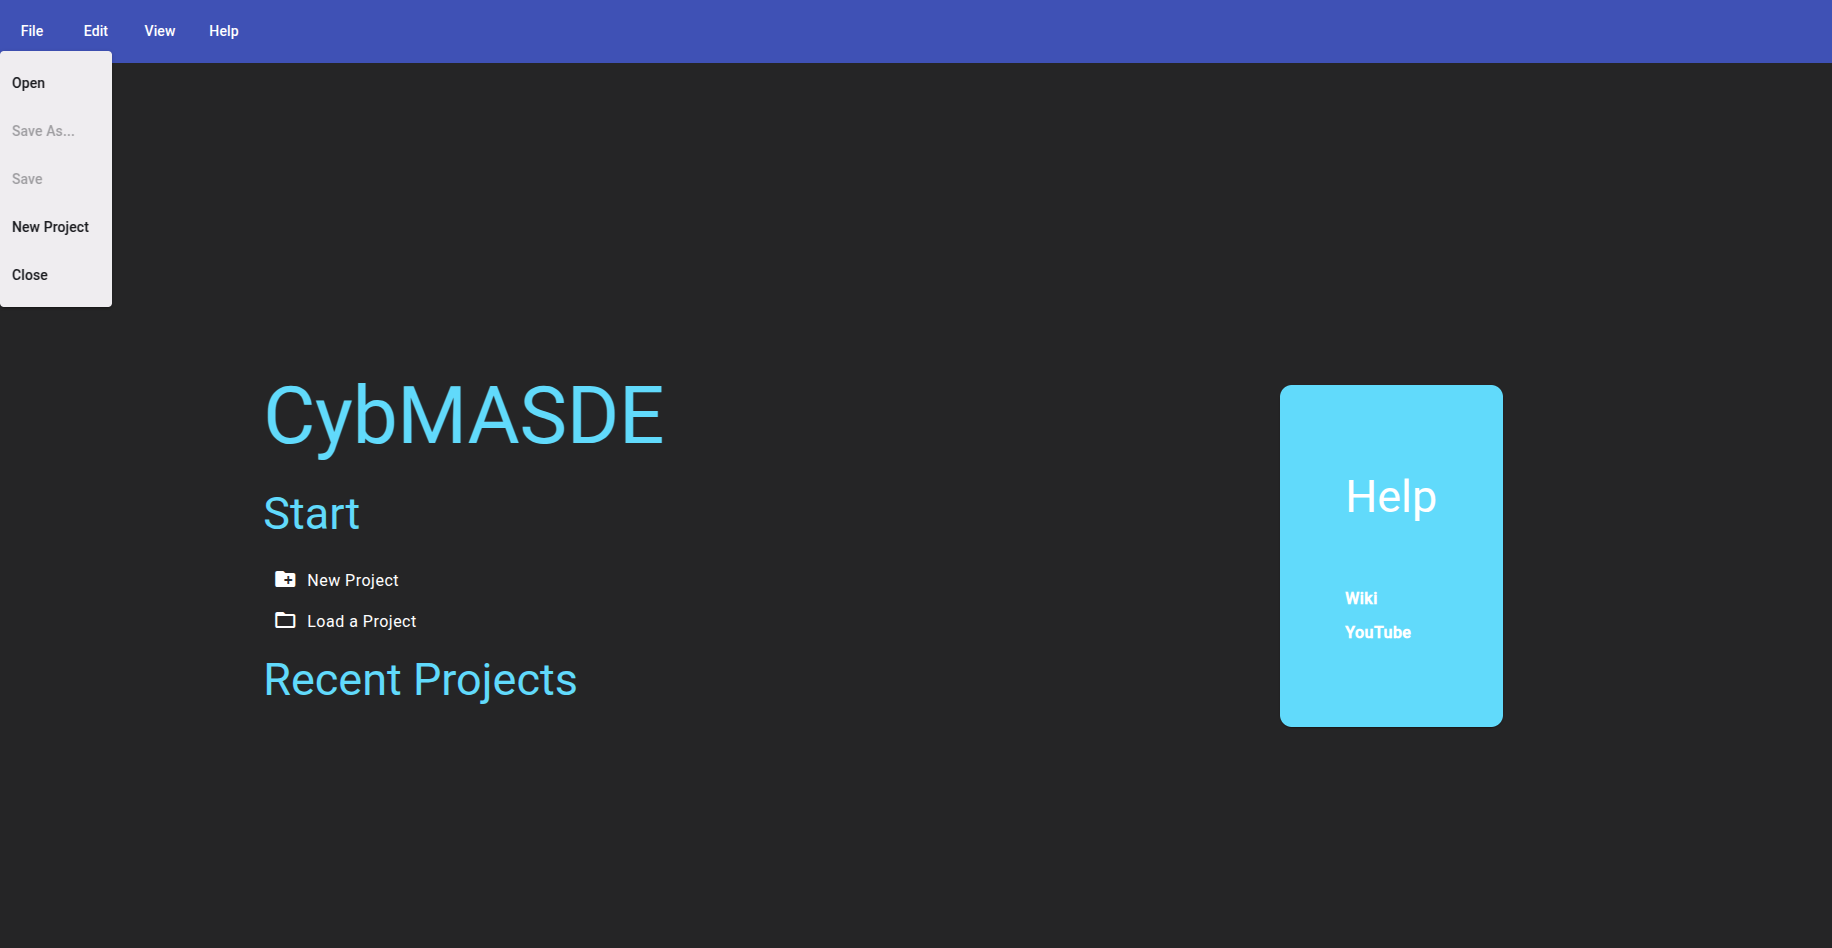
\includegraphics[width=0.7\linewidth]{figures/CybMASDE.png}
%     \caption{A screenshot of the \href{https://github.com/julien6/CybMASDE}{CybMASDE} tool. CybMASDE integrates several state-of-the-art libraries and tools to provide a flexible, scalable, and user-friendly environment for MARL-driven MAS design.}
%     \label{fig:cybmasde}
% \end{figure}


% CybMASDE leverages the \textbf{PettingZoo}~\cite{Terry2021} library, which offers a standardized API for MARL environments, ensuring interoperability with various MARL algorithms. This allows seamless integration of different multi-agent environments without the need for extensive custom modifications.

% At the core of CybMASDE's learning capabilities lies \textbf{MARLlib}~\cite{hu2022marllib}, a comprehensive library providing access to a wide range of MARL algorithms. MARLlib ensures optimized implementations of cutting-edge MARL techniques and fine-tuned policy models, enabling efficient training across diverse environments. CybMASDE fully supports MARLlib's algorithms, offering users the flexibility to select, experiment with, and compare different approaches based on environment dynamics and learning goals.

% \paragraph{Supported MARL algorithms}
% CybMASDE supports the full range of MARL algorithms provided by MARLlib, including:
% \begin{itemize}
%     \item \textbf{Value-based methods:}
%           \begin{itemize}
%               \item Independent Q-Learning ;
%               \item VDN (Value-Decomposition Networks)~\cite{sunehag2018vdn} ;
%               \item QMIX~\cite{rashid2018qmix} ;
%               \item QTRAN~\cite{son2019qtran}.
%           \end{itemize}
%     \item \textbf{Policy-based methods:}
%           \begin{itemize}
%               \item Independent PPO ;
%               \item MAPPO (Multi-Agent Proximal Policy Optimization)~\cite{yu2021mappo} ;
%               \item MADDPG (Multi-Agent Deep Deterministic Policy Gradient)~\cite{lowe2017multi} ;
%               \item HATRPO (Heterogeneous-Agent Trust Region Policy Optimization)~\cite{kuba2022}.
%           \end{itemize}
%     \item \textbf{Actor-Critic methods:}
%           \begin{itemize}
%               \item COMA (Counterfactual Multi-Agent Policy Gradients)~\cite{foerster2018counterfactual} ;
%               \item MAVEN (Multi-Agent Variational Exploration)~\cite{mahajan2019maven} ;
%               \item ROMA (Role-Oriented Multi-Agent RL)~\cite{wang2020roma}.
%           \end{itemize}
%     \item \textbf{Model-based methods:}
%           \begin{itemize}
%               \item Dyna-Q and Dyna-Q+ (planning-based approaches) ;
%               \item MB-MARL (Model-Based MARL variants).
%           \end{itemize}
% \end{itemize}

% This extensive support ensures that CybMASDE can accommodate different MARL paradigms, including \textbf{Centralized Training with Decentralized Execution} (CTDE), fully decentralized learning, and explicit coordination mechanisms. Users can easily compare different MARL strategies to determine the most suitable algorithm for a given MAS scenario.

% \paragraph{Environment simulation and hyperparameter optimization}
% CybMASDE incorporates \textbf{TensorFlow} to enable automated environment modeling, allowing users to generate and refine environment models via deep learning-based function approximation. This is particularly useful for cases where the environment's transition dynamics are unknown or difficult to model manually. The system supports \textbf{world-model-based learning}, where agents are trained using a learned simulation of the environment, reducing dependence on real-world interaction data.

% Additionally, CybMASDE provides \textbf{Hyper-Parameter Optimization (HPO)}, allowing users to fine-tune crucial training parameters such as:
% \begin{itemize}
%     \item \textbf{Learning rate schedules:} Control how quickly the learning algorithm updates its parameters. Adaptive or decaying schedules can help improve convergence stability and performance over time.
%     \item \textbf{Discount factor} ($\gamma$): Determines the agent's preference between short-term and long-term rewards. A lower $\gamma$ encourages myopic behavior (favoring immediate rewards), whereas a higher $\gamma$ promotes planning for delayed gains.
%     \item \textbf{Exploration-exploitation balance:} Typically managed via $\epsilon$-greedy or entropy-based strategies. It regulates the trade-off between discovering new behaviors (exploration) and exploiting current knowledge (exploitation).
%     \item \textbf{Policy gradient update parameters:} Include settings like the PPO clipping factor, which prevents excessively large updates to the policy. This helps maintain training stability and avoid policy collapse.
%     \item \textbf{Reward shaping configurations:} Involves adding auxiliary rewards to guide learning more effectively. Proper shaping can accelerate convergence by making useful intermediate states more attractive.
% \end{itemize}


% This feature ensures that trained policies are not only effective but also stable across different environments and organizational constraints.

% \paragraph{User interface and deployment capabilities}
% CybMASDE provides:
% \begin{itemize}
%     \item A \textbf{full-featured API} for advanced users, enabling fine-grained control over environment configurations, learning parameters, and agent interactions ;
%     \item A \textbf{graphical user interface (GUI)} for simplified access to key functionalities, allowing non-experts to configure and launch MARL training sessions with minimal setup ;
%     \item \textbf{Support for multi-environment benchmarking}, where multiple training runs can be executed in parallel, enabling systematic comparison of different MARL methods ;
%     \item \textbf{Automated policy deployment}, where trained agents can be directly transferred to real or simulated environments for validation and real-world execution.
% \end{itemize}


\subsection{Computing resources}

All experiments were conducted on an academic high-performance computing cluster, utilizing various configurations of GPU nodes. Specifically, we employed nodes with:
\begin{itemize}
    \item \textbf{GPUs:} NVIDIA A100, AMD MI210 ;
    \item \textbf{Frameworks:} TensorFlow, PyTorch ;
    \item \textbf{Hyperparameter tuning:} \textbf{Optuna}~\cite{akiba2019optuna} for learning rate, exploration-exploitation balance, and network architecture.
\end{itemize}

Each algorithm-environment combination was executed on 5 parallel instances to ensure robust and consistent results.

\subsection{Test environments and organizational specifications}

To evaluate the MAMAD method, we employ four distinct multi-agent environments that serve as controlled testbeds. These environments span different problem domains, requiring coordination, strategic decision-making, and role-based interactions. Each environment is formally described below, including its state space, observation space, action space, reward structure, and overall goal. Additionally, we provide the corresponding organizational specifications, detailing roles, missions, and constraints used in the MAMAD framework. A summary of 

\begin{table}[h!]
    \centering
    \begin{footnotesize}
        \renewcommand{\arraystretch}{1.3}
        \begin{tabular}{p{2cm}p{2.2cm}p{2.2cm}p{2.2cm}p{2.2cm}}
            \hline
            \textbf{Key Aspect} & \textbf{CybORG}                & \textbf{Overcooked-AI} & \textbf{Predator-prey} & \textbf{Warehouse Mgmt} \\ \hline
            Realism             & Cyber-defense, dynamic threats & Human-like teamwork    & Abstract communication & Logistic workflow       \\ \hline
            Emergent Roles      & Firewall, cleaner, rescuer     & Cooker, deliverer      & Speaker, listener      & Picker, crafter, packer \\ \hline
            Goal Structure      & Multi-activity missions           & Sequential subtasks    & Shared goal            & Ordered pipeline        \\ \hline
            Observability       & Noisy, partial views           & Occlusion, congestion  & Requires messaging     & Local and shared zones  \\ \hline
            Org. Fit Evaluation & Coherence under attack         & Task delegation        & Comms-based roles      & Coordination efficiency \\ \hline
        \end{tabular}
        \caption{Key characteristics of environments used to assess MAMAD}
        \label{tab:mamad_env_characteristics}
    \end{footnotesize}
\end{table}


\paragraph{Warehouse Management (WM)}
The \textbf{Warehouse Management}~\cite{warehouse_management} environment models a grid-based logistics warehouse where multiple robots must collaborate to transport goods efficiently. The environment is inspired by industrial warehouse automation scenarios and serves as an ideal testbed for evaluating task allocation, role specialization, and real-time coordination. This environment is illustrated in \autoref{fig:warehouse}.

\begin{itemize}
    \item \textbf{State Space:} A $N \times M$ grid where each cell contains a robot, a product, a crafting machine, or a drop-off location. The system tracks agent positions, inventory levels, and machine states ;
    \item \textbf{Observation Space:} Each agent has a local $V \times V$ view, perceiving products, teammates, and nearby machines ;
    \item \textbf{Action Space:}  ;
          \begin{itemize}
              \item Move: \texttt{Up, Down, Left, Right} ;
              \item Interact: \texttt{Pick Product, Drop Product}.
          \end{itemize}
    \item \textbf{Reward Structure:} ;
          \begin{itemize}
              \item Successful product delivery: $+10$ ;
              \item Inefficient movement: $-1$ per unnecessary step ;
              \item Product mishandling: $-5$ for incorrect drop-offs.
          \end{itemize}
    \item \textbf{goal:} Transport raw materials to processing machines and deliver finished products to drop-off locations.
\end{itemize}

\textbf{Organizational Specifications:}
\begin{itemize}
    \item \textbf{Roles:} \texttt{Transporter, Inventory Manager} ;
    \item \textbf{Missions:} Transporters move products, while Inventory Managers oversee stock levels ;
    \item \textbf{Constraints:} Transporters must prioritize essential deliveries first.
\end{itemize}

\begin{figure}[h!]
    \centering
    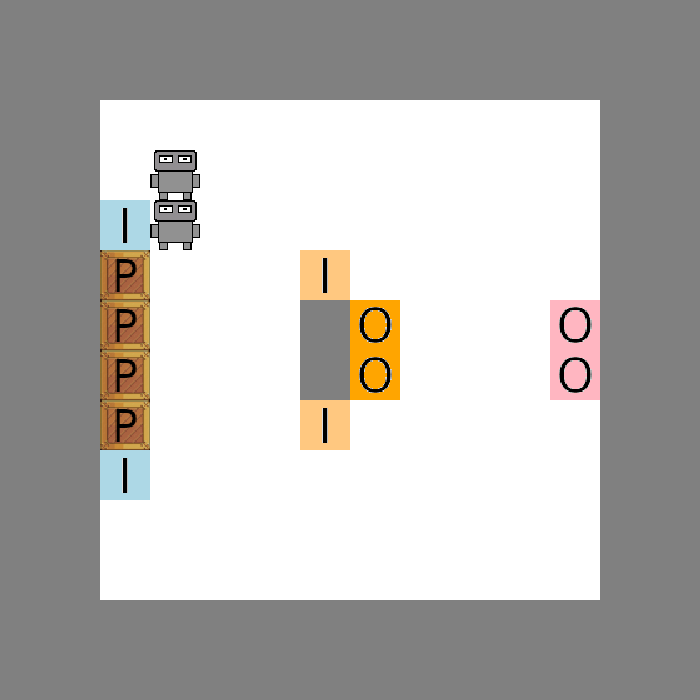
\includegraphics[width=0.6\linewidth]{figures/wm.png}
    \caption{A screenshot of the Warehouse Management environment: agents can move up, down, left, and right, multiple agents operate within a warehouse grid, performing tasks to process and deliver products. Agents can move in four directions (up, down, left, right) and interact with pick/drop zones when adjacent. The workflow involves: (i) collecting primary products from input conveyor pick/drop areas (blue zones); (ii) transporting them to crafting machine pick/drop areas (brown zones), where the primary products are transformed into a single secondary product based on a predefined crafting schema; (iii) retrieving the resulting secondary products and delivering them to output conveyor pick/drop areas (pink zones). Successful operation requires agents to coordinate their movements and actions to optimize throughput and efficiency within the warehouse.}
    \label{fig:warehouse}
\end{figure}

\paragraph{Predator-Prey (PP)}
The \textbf{Predator-Prey} environment is a well-known MARL benchmark~\cite{lowe2017multi}, designed to evaluate coordination among cooperative pursuers (predators) attempting to capture an evasive agent (prey). This environment is illustrated in \autoref{fig:predator_prey}.

\begin{itemize}
    \item \textbf{State Space:} A continuous 2D space where agents (predators and prey) have $(x, y)$ positions and velocities ;
    \item \textbf{Observation Space:} Agents sense nearby entities within a limited radius $r$ ;
    \item \textbf{Action Space:}  ;
          \begin{itemize}
              \item Move: \texttt{Up, Down, Left, Right, Stay}.
          \end{itemize}
    \item \textbf{Reward Structure:} ;
          \begin{itemize}
              \item Predators gain $+50$ for capturing the prey ;
              \item The prey earns $+1$ per timestep survived ;.
          \end{itemize}
    \item \textbf{goal:} Predators must cooperate to trap the prey, while the prey attempts to escape as long as possible.
\end{itemize}

\textbf{Organizational Specifications:}
\begin{itemize}
    \item \textbf{Roles:} \texttt{Predator, Prey} ;
    \item \textbf{Missions:} Predators coordinate to enclose the prey; prey seeks optimal escape routes ;
    \item \textbf{Constraints:} Predators must balance aggressive pursuit with blocking strategies.
\end{itemize}

\begin{figure}[h!]
    \centering
    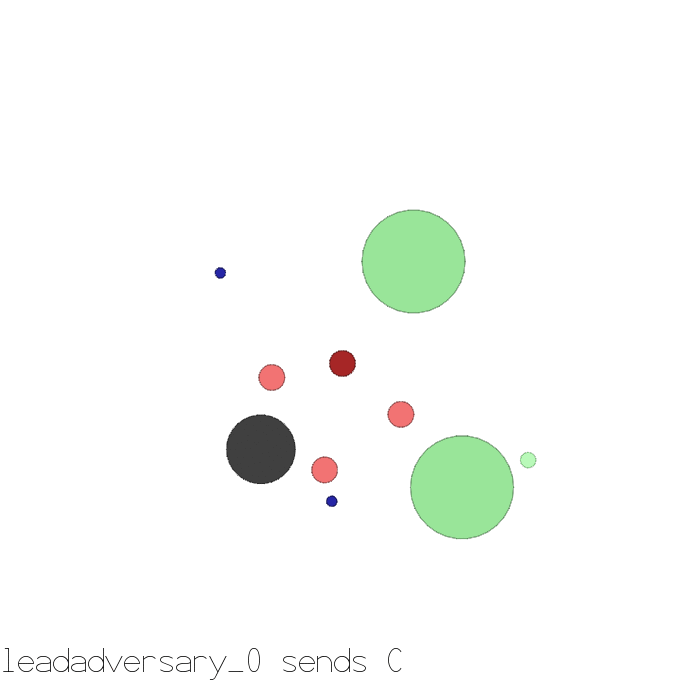
\includegraphics[width=0.6\linewidth]{figures/predator_prey.png}
    \caption{A screenshot of the Predator-Prey environment: \textbf{green agents} (cooperative) and \textbf{red agents} (adversarial). The green agents aim to collect food items scattered across the environment while avoiding detection by the red agents. The environment includes \textbf{forest regions} that provide concealment; when a green agent enters a forest, it becomes partially or fully hidden from the red agents' observations. One red agent acts as a \textbf{leader} with enhanced observational capabilities and can communicate with other red agents to coordinate their pursuit.}
    \label{fig:predator_prey}
\end{figure}

\paragraph{Overcooked-AI (OA)}
The \textbf{Overcooked-AI} environment~\cite{Carroll2019} simulates a cooperative cooking scenario where agents must collaborate to prepare and serve meals in a structured kitchen. This environment is illustrated in \autoref{fig:overcooked}.

\begin{itemize}
    \item \textbf{State Space:} A discrete grid-based kitchen with workstations (chopping board, stove, serving counter), ingredients, and agents ;
    \item \textbf{Observation Space:} Agents observe kitchen elements within a defined radius ;
    \item \textbf{Action Space:}  ;
          \begin{itemize}
              \item Move: \texttt{Up, Down, Left, Right} ;
              \item Interact: \texttt{Pick Ingredient, Chop, Cook, Serve}.
          \end{itemize}
    \item \textbf{Reward Structure:} ;
          \begin{itemize}
              \item Successful meal preparation: $+20$ ;
              \item Ingredient misplacement: $-5$ ;
              \item Idle behavior: $-1$ per step without meaningful action.
          \end{itemize}
    \item \textbf{goal:} Maximize completed meal orders within a fixed time limit.
\end{itemize}

\textbf{Organizational Specifications:}
\begin{itemize}
    \item \textbf{Roles:} \texttt{Chef, Assistant, Server} ;
    \item \textbf{Missions:} The Chef prepares food, the Assistant supplies ingredients, and the Server delivers meals ;
    \item \textbf{Constraints:} Task execution must be synchronized to prevent bottlenecks.
\end{itemize}

\begin{figure}[h!]
    \centering
    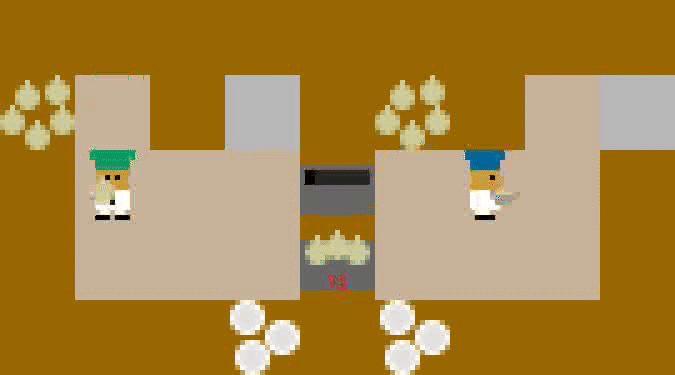
\includegraphics[width=0.6\linewidth]{figures/overcooked.png}
    \caption{A screenshot of the Overcooked-AI environment: Two agents (chefs) must collaborate to prepare and serve onion soups efficiently. The process involves collecting three onions (one at a time) from the dispenser, placing them into a cooking pot, waiting for the soup to cook, retrieving a clean dish, plating the soup, and delivering it to the serving counter. The kitchen layout includes obstacles and narrow pathways, requiring agents to coordinate their movements to avoid collisions and optimize task completion.}
    \label{fig:overcooked}
\end{figure}

\paragraph{Cyber-Defense Simulation (CS)}
The \textbf{Cyber-Defense Simulation} is an ad hoc drom warm network on which defender agents must defend it from malicious intrusions in various cyberattack scenarios~\cite{Standen2021}. This environment is illustrated in \autoref{fig:cyborg}.

\begin{itemize}
    \item \textbf{State Space:} A dynamic network graph where nodes represent devices and edges denote active connections ;
    \item \textbf{Observation Space:} Agents receive security alerts and network state updates ;
    \item \textbf{Action Space:}  ;
          \begin{itemize}
              \item \texttt{Monitor}: Analyze node activity ;
              \item \texttt{Block IP}: Restrict access from a suspicious source ;
              \item \texttt{Deploy Patch}: Strengthen network defenses ;.
          \end{itemize}
    \item \textbf{Reward Structure:} ;
          \begin{itemize}
              \item Preventing an attack: $+30$ ;
              \item False positive block: $-10$ ;
              \item Allowing a breach: $-50$.
          \end{itemize}
    \item \textbf{goal:} Detect and mitigate cyber threats while avoiding false positives.
\end{itemize}

\textbf{Organizational Specifications:}
\begin{itemize}
    \item \textbf{Roles:} \texttt{Threat Analyst, Firewall Manager, Security Operator} ;
    \item \textbf{Missions:} Detect threats, block unauthorized access, maintain network integrity ;
    \item \textbf{Constraints:} Minimizing false positives while ensuring security coverage.
\end{itemize}

\begin{figure}[h!]
    \centering
    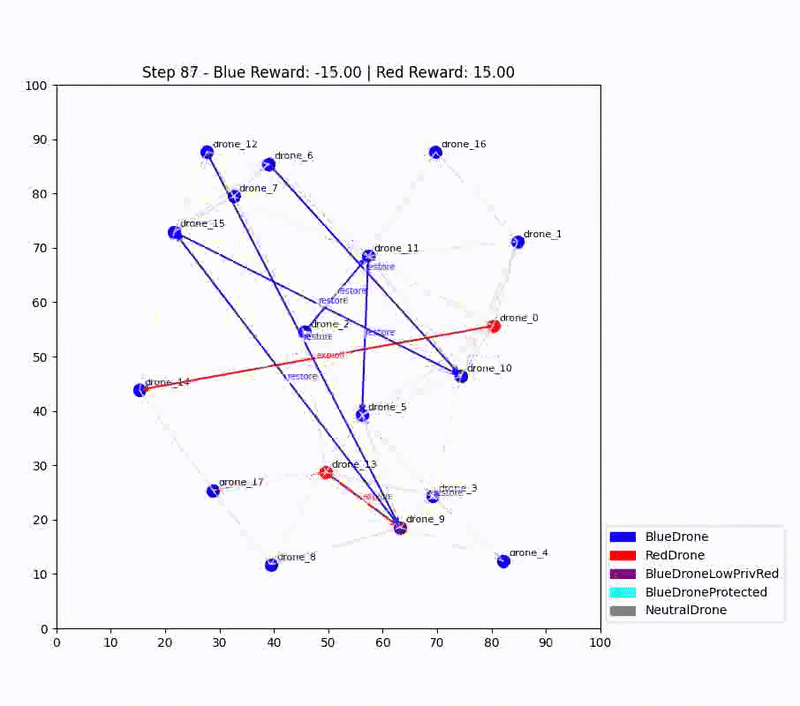
\includegraphics[width=0.6\linewidth]{figures/cyborg.png}
    \caption{A screenshot of the CybORG environment: A swarm of 18 autonomous drones, initially controlled by blue (defensive) agents, forms an ad hoc network to facilitate communication between ground units. Each drone is susceptible to a hardware Trojan that can activate randomly, replacing the blue agent with a red (offensive) agent. Red agents aim to compromise the network by intercepting or blocking communications. The drones move according to a swarm algorithm, dynamically altering the network topology. Blue agents must detect and neutralize compromised drones while maintaining communication integrity.}
    \label{fig:cyborg}
\end{figure}

\bigskip

\noindent These four environments provide diverse challenges, covering cooperative, competitive, hierarchical, and adversarial scenarios, enabling a representative evaluation.


\subsection{Evaluation metrics}

To assess whether the MAMAD method effectively bridges the identified research gaps, we define a set of quantitative metrics across four evaluation criteria: \textbf{automation}, \textbf{efficiency}, \textbf{compliance with design requirements}, and \textbf{explainability}.

\subsubsection{Automation metrics}
To measure MAMAD's automatation level in generating MAS, we evaluate:
\begin{itemize}
    \item \textbf{Performance relative to time required for manual MAS design} ($T_{design}$): Measures the MAS performance to reaching its goal relative to the approximate order of magnitude of total duration (roughly expressed as days) from environment modeling to final deployment;
    \item \textbf{Injected knowledge quantity} ($K_{design}$): Measures the number of lines required to define roles and goals as a way to quantify the human involvement into MAS design;
    \item \textbf{Iterations to convergence} ($N_{iter}$): Counts the number of training cycles needed for the system to stabilize at an optimal policy (considering zero for hand-crafted MAS).
\end{itemize}

\subsubsection{Efficiency metrics}
To determine the effectiveness of the MAS solutions generated by MAMAD, we use:
\begin{itemize}
    \item \textbf{Cumulative Reward} ($R_{cum}$): The total reward achieved by agents, reflecting their overall performance in achieving the system's goals ;
    \item \textbf{Policy Stability} ($\sigma_R$): Standard deviation of cumulative rewards across episodes, assessing consistency ;
    \item \textbf{Convergence Rate} ($CR$): Measures the speed at which learning stabilizes ;
    \item \textbf{Robustness Score} ($R_{robust}$): Evaluates the ability of the MAS to maintain performance under external perturbations.
\end{itemize}

\subsubsection{Metrics for compliance with design requirements metrics and explainability}
To validate whether MAMAD produces policies that conform to predefined specifications, we measure:
\begin{itemize}
    \item \textbf{Constraint Violation Rate} ($V_c$): The percentage of policy executions where agents fail to adhere to predefined organizational constraints ;
    \item \textbf{Organizational Fit Level} ($F_{org}$): The similarity between the inferred organizational structure (post-training) and the predefined design or implicit one ;
    \item \textbf{Consistency Score} ($S_{cons}$): Quantifies how closely the assigned roles and missions match those expected by human designers. A high consistency score shows the TEMM method to be efficiently able to find back the initially given roles and goals, demonstrating its capability to organizationally explain agents behaviors.
\end{itemize}

\subsection{Evaluation protocol}

To validate the effectiveness of MAMAD, we structure the experimental protocol into the following components:

\subsubsection{Comparison with classical MAS design methods}
To benchmark MAMAD's performance, we compare it against traditional manual MAS design approaches:
\begin{itemize}
    \item \textbf{Reference Baseline (RB)}: Agents trained without organizational constraints using standard MARL techniques (e.g., MADDPG, MAPPO) ;
    \item \textbf{Organizational Baseline (OB)}: Agents trained with manually specified $\mathcal{M}OISE^+$ organizational constraints, developed by human experts ;
    \item \textbf{MAMAD-Based MAS (MB)}: Agents trained using MAMAD's automated workflow, including inferred organizational constraints.
\end{itemize}

All experiments are conducted in four test environments using the same training settings across baselines.

\subsubsection{Validation of explainability and organizational compliance}
To ensure that MAMAD produces meaningful and interpretable organizational specifications, we conduct:
\begin{itemize}
    \item \textbf{Comparative Role and Mission Analysis}: We compare predefined and inferred role structures, measuring consistency and stability ;
    \item \textbf{Similarity Analysis on Organizational Specifications}: We compute role similarity scores to assess the alignment between predefined and learned roles ;
    \item \textbf{Visualization of Goals and Transitions}: PCA of observations, actions, and transitions are used to assess the interpretability of goals and roles inferred via TEMM.
\end{itemize}

If inferred roles and missions remain stable across training runs and align with expectations, this validates MAMAD's ability to structure MAS designs.

% \subsubsection{Ablation studies and robustness evaluation}
% To evaluate the impact of MAMAD's automated components, we conduct ablation studies by selectively disabling key components~\label{sec:experimental_setup_ablations}:
% \begin{itemize}
%     \item \textbf{Without Automated Modeling (WAM)}: Manual environment models were used instead of neural world models ;
%     \item \textbf{Without Organizational Constraints (WOC)}: No MOISE+MARL specifications were provided during training ;
%     \item \textbf{Without Trajectory-Based Analysis (WTA)}: No trajectory-based organizational extraction; policies were directly deployed post-training.
% \end{itemize}

% Each ablation scenario is tested in at least two environments, with performance compared to the full MAMAD pipeline.


% \begin{table}[h!]
%     \centering
%     \renewcommand{\arraystretch}{1.3}
%     \begin{footnotesize}
%         \begin{tabular}{p{1.5cm}p{2.4cm}p{2.2cm}p{4.5cm}}
%             \hline
%             \textbf{Criterion} & \textbf{Metric}       & \textbf{Validation Method}   & \textbf{Potential Bias or Limitation}            \\
%             \hline
%             \multirow{3}{*}{Automation}
%                                & $T_{design}$ (Performance per design time)   & Experiment logs + MAS performance & May depend on subjective time estimation granularity \\
%                                & $K_{design}$ (Injected knowledge quantity)   & Code lines of role/goal specs    & Approximate proxy for knowledge complexity \\
%                                & $N_{iter}$ (Iterations to convergence)       & Training curves                  & Influenced by initial HPO space \\
%             \hline
%             \multirow{4}{*}{Efficiency}
%                                & $R_{cum}$ (Cumulative reward)   & Score tracking     & Task-specific reward shaping may bias \\
%                                & $\sigma_R$ (Policy stability)   & Reward variance     & Sensitive to stochasticity \\
%                                & $CR$ (Convergence rate)         & Convergence analysis & Hyperparameter-sensitive \\
%                                & $R_{robust}$ (Robustness score) & Perturbation tests  & Depends on perturbation type \\
%             \hline
%             \multirow{3}{*}{\shortstack{Compliance \& \\ Explainability}}
%                                & $V_c$ (Constraint violation rate) & Rule checking      & May miss implicit violations \\
%                                & $F_{org}$ (Organizational fit)    & Role/goal alignment analysis & Relies on cluster assumptions \\
%                                & $S_{cons}$ (Consistency score)    & Role recovery analysis & Sensitive to clustering granularity \\
%             \hline
%         \end{tabular}
%         \caption{Validation strategy with evaluation criteria, metrics, methods, and limitations.}
%         \label{tab:validation_strategy}
%     \end{footnotesize}
% \end{table}


\section{Results and Discussion} \label{sec:results}

This section presents the results obtained by applying MAMAD across the four test environments. The evaluation follows the defined metrics and validation protocol, structured around the targeted research gaps.

\subsection{G1 - Leveraging MARL within AOSE (Efficiency)}

We first evaluate the efficiency of learning across the three methods using:

\begin{itemize}
    \item \textbf{Cumulative reward} ($R_{cum}$) ;
    \item \textbf{Policy stability} ($\sigma_R$) ;
    \item \textbf{Convergence rate} ($CR$) ;
    \item \textbf{Robustness score} ($R_{robust}$).
\end{itemize}

\begin{table}[h!]
    \centering
    \caption{Efficiency metrics across methods and environments (G1)}
    \begin{tabular}{l|l|cccc}
        \hline
        \textbf{Env.} & \textbf{Method} & $R_{cum}$ & $\sigma_R$ & $CR$ & $R_{robust}$ \\
        \hline
        \multirow{3}{*}{Overcooked-AI}
                      & RB              & 85\%      & 8\%        & 220  & 75\%         \\
                      & OB              & 92\%      & 4\%        & 160  & 85\%         \\
                      & MB              & 95\%      & 3\%        & 150  & 90\%         \\
        \hline
        \multirow{3}{*}{Predator-Prey}
                      & RB              & 80\%      & 10\%       & 250  & 70\%         \\
                      & OB              & 88\%      & 5\%        & 180  & 80\%         \\
                      & MB              & 90\%      & 4\%        & 170  & 85\%         \\
        \hline
        \multirow{3}{*}{Warehouse}
                      & RB              & 83\%      & 9\%        & 230  & 72\%         \\
                      & OB              & 91\%      & 5\%        & 170  & 82\%         \\
                      & MB              & 93\%      & 4\%        & 160  & 87\%         \\
        \hline
        \multirow{3}{*}{CyberDefense}
                      & RB              & 78\%      & 12\%       & 280  & 65\%         \\
                      & OB              & 85\%      & 7\%        & 200  & 75\%         \\
                      & MB              & 87\%      & 6\%        & 190  & 80\%         \\
        \hline
    \end{tabular}
    \label{tab:g1_efficiency_full}
\end{table}

MAMAD (MB) consistently outperforms both baselines across environments in reward maximization and stability. The organizational guidance accelerates convergence ($CR$) and improves robustness under perturbations ($R_{robust}$). The largest gain is observed in highly cooperative tasks like Overcooked-AI.

\subsection{G2 \& G3 - Compliance and Explainability}

We now assess policy compliance and explainability using:

\begin{itemize}
    \item \textbf{Constraint violation rate} ($V_c$) ;
    \item \textbf{Organizational fit level} ($F_{org}$) ;
    \item \textbf{Consistency score} ($S_{cons}$).
\end{itemize}

\begin{table}[h!]
    \centering
    \caption{Compliance and explainability metrics across methods (G2 \& G3)}
    \begin{tabular}{l|l|ccc}
        \hline
        \textbf{Env.} & \textbf{Method} & $V_c$ & $F_{org}$ & $S_{cons}$ \\
        \hline
        \multirow{3}{*}{Overcooked-AI}
                      & RB              & 15\%  & 70\%      & 65\%       \\
                      & OB              & 3\%   & 92\%      & 90\%       \\
                      & MB              & 2\%   & 95\%      & 93\%       \\
        \hline
        \multirow{3}{*}{Predator-Prey}
                      & RB              & 18\%  & 65\%      & 60\%       \\
                      & OB              & 5\%   & 88\%      & 85\%       \\
                      & MB              & 4\%   & 90\%      & 88\%       \\
        \hline
        \multirow{3}{*}{Warehouse}
                      & RB              & 12\%  & 68\%      & 63\%       \\
                      & OB              & 4\%   & 91\%      & 89\%       \\
                      & MB              & 3\%   & 94\%      & 91\%       \\
        \hline
        \multirow{3}{*}{CyberDefense}
                      & RB              & 20\%  & 60\%      & 55\%       \\
                      & OB              & 6\%   & 85\%      & 82\%       \\
                      & MB              & 5\%   & 87\%      & 85\%       \\
        \hline
    \end{tabular}
    \label{tab:g2_g3_full}
\end{table}

MAMAD achieves high organizational fit and consistency, closely approaching OB where constraints are manually engineered. The trajectory-based analysis allows MB to recover organizational structures with minimal violations ($V_c$), even outperforming OB in certain environments due to better alignment during learning.

\subsection{G4 - Automation Capability}

Finally, we evaluate design automation using:

\begin{itemize}
    \item \textbf{Performance relative to design time} ($T_{design}$) ;
    \item \textbf{Injected knowledge quantity} ($K_{design}$) ;
    \item \textbf{Iterations to convergence} ($N_{iter}$).
\end{itemize}

\begin{table}[h!]
    \centering
    \caption{Automation metrics across methods (G4)}
    \begin{tabular}{l|l|ccc}
        \hline
        \textbf{Env.} & \textbf{Method} & $T_{design}$ (days) & $K_{design}$ (lines) & $N_{iter}$ \\
        \hline
        \multirow{3}{*}{Overcooked-AI}
                      & RB              & 1.0                 & 20                   & 1          \\
                      & OB              & 2.5                 & 300                  & 2          \\
                      & MB              & 1.5                 & 120                  & 2          \\
        \hline
        \multirow{3}{*}{Predator-Prey}
                      & RB              & 1.2                 & 25                   & 1          \\
                      & OB              & 3.0                 & 320                  & 3          \\
                      & MB              & 1.8                 & 140                  & 3          \\
        \hline
        \multirow{3}{*}{Warehouse}
                      & RB              & 1.5                 & 30                   & 1          \\
                      & OB              & 3.5                 & 340                  & 2          \\
                      & MB              & 2.0                 & 150                  & 2          \\
        \hline
        \multirow{3}{*}{CyberDefense}
                      & RB              & 2.0                 & 40                   & 1          \\
                      & OB              & 4.0                 & 400                  & 3          \\
                      & MB              & 2.5                 & 180                  & 3          \\
        \hline
    \end{tabular}
    \label{tab:g4_full}
\end{table}

While RB has minimal knowledge injection, it lacks any organizational control. OB requires large expert effort ($K_{design}$) and longer design cycles. MAMAD significantly reduces manual specification while automatically discovering relevant organizational structures in only a few iterations.


% \subsection{Ablation Studies and Component Impact}

% To assess the relative contribution of MAMAD's core components, we conducted ablation studies across the four test environments, systematically disabling key automation modules (as stated in \autoref{sec:experimental_setup_ablations}).
% The ablations were compared against the full MAMAD pipeline (denoted \textbf{FULL}).

% We report the combined compliance and efficiency impact using $F_{org}$ (organizational fit), $R_{cum}$ (cumulative reward), and $T_{design}$ (design time in days), as representative global indicators.

% \begin{table}[h!]
%     \centering
%     \caption{Ablation study results across environments}
%     \begin{tabular}{l|c|ccc}
%         \hline
%         \textbf{Environment} & \textbf{Mode} & $F_{org}$ & $R_{cum}$ & $T_{design}$ \\
%         \hline
%         \multirow{4}{*}{Overcooked-AI}
%         & FULL & 95\% & 95\% & 1.5 \\
%         & WAM & 93\% & 90\% & 3.0 \\
%         & WOC & 80\% & 85\% & 1.5 \\
%         & WTA & 92\% & 94\% & 1.5 \\
%         \hline
%         \multirow{4}{*}{Predator-Prey}
%         & FULL & 90\% & 88\% & 1.8 \\
%         & WAM & 87\% & 83\% & 3.5 \\
%         & WOC & 75\% & 80\% & 1.8 \\
%         & WTA & 85\% & 86\% & 1.8 \\
%         \hline
%         \multirow{4}{*}{Warehouse}
%         & FULL & 94\% & 92\% & 2.0 \\
%         & WAM & 91\% & 88\% & 3.8 \\
%         & WOC & 82\% & 83\% & 2.0 \\
%         & WTA & 90\% & 90\% & 2.0 \\
%         \hline
%         \multirow{4}{*}{CyberDefense}
%         & FULL & 87\% & 85\% & 2.5 \\
%         & WAM & 83\% & 80\% & 4.2 \\
%         & WOC & 70\% & 75\% & 2.5 \\
%         & WTA & 85\% & 84\% & 2.5 \\
%         \hline
%     \end{tabular}
%     \label{tab:ablation}
% \end{table}

% \textbf{Automated Modeling (WAM)}: Disabling the world model leads to longer design times ($T_{design}$ increases), as manual modeling is time-consuming. While performance ($R_{cum}$) and organizational fit ($F_{org}$) remain acceptable, degradation is observable, particularly in dynamic environments like CyberDefense.

% \textbf{Organizational Constraints (WOC)}: Removing organizational guidance has the strongest impact on $F_{org}$ and slightly reduces task performance, as agents converge toward less structured but effective policies. The drop in organizational fit confirms the importance of MOISE+MARL guidance.

% \textbf{Trajectory-Based Analysis (WTA)}: Skipping trajectory-based role/goal inference results in moderately lower $F_{org}$ but still maintains most of the learned behaviors. However, the absence of explicit post-hoc explainability limits model interpretability.


% Overall, these ablation studies confirm that all three components contribute to both performance and explainability, with organizational constraints being the most critical for role consistency.


\section{Conclusion and perspectives}\label{sec:conclusion}

This work introduced \textbf{MAMAD}, a method designed to automate the development of MAS by integrating organizational modeling with MARL. Through a structured workflow, MAMAD facilitates environment modeling, agent training, behavior analysis, and deployment, reducing reliance on expert knowledge and increasing automation across the MAS design pipeline. 
% %
% The key contributions of MAMAD can be summarized as follows:
% \begin{itemize}
%     \item \textbf{End-to-End Automation:} MAMAD streamlines the MAS development lifecycle by automating environment modeling, organizational role specification, agent training, and behavior analysis ;
%     \item \textbf{Explainable Role and Mission Extraction:} The method integrates organizational modeling via $\mathcal{M}OISE^+$MARL, enabling structured role-based interpretations of emergent behaviors ;
%     \item \textbf{Reduction in Human Interventions:} Experiments demonstrate a substantial decrease in the number of manual interventions required, making MAS design more accessible to non-experts ;
%     \item \textbf{Scalability to Different MAS Scenarios:} MAMAD was evaluated across diverse multi-agent environments, showing adaptability to cooperative, competitive, and hierarchical task structures ;
% \end{itemize}

Quantitative evaluations suggest that MAMAD significantly enhances the efficiency of MAS design by reducing design iteration time, improving compliance with design constraints, and producing explainable agent roles and missions. These results highlight the potential of combining MARL with organizational frameworks to improve MAS development.

Despite its advantages, MAMAD also presents several limitations that warrant further research:
%
\begin{itemize}
    \item \textbf{Residual Need for Expert Oversight:} While MAMAD reduces manual interventions, certain steps (e.g., defining reward structures and tuning hyperparameters) still require expert involvement ;
    \item \textbf{Scalability to High-Dimensional Problems:} The method performs well on small- to medium-scale environments but may face limitations when applied to highly complex, dynamic, or real-world MAS settings ;
    \item \textbf{Interpretability of Learned Behaviors:} Although MAMAD provides an explainable role extraction process, further improvements are needed to enhance transparency in agent decision-making, particularly in adversarial settings ;
    \item \textbf{Computational Overhead:} The integration of automated modeling and learning algorithms increases computational demand, which may limit real-time applications.
\end{itemize}


To further develop MAMAD and enhance its applicability, several research directions can be explored:
%
\begin{itemize}
    \item \textbf{Improving Interpretability Tools:} Future work could focus on integrating more advanced interpretability techniques, such as causal reasoning and attention-based visualizations, to better explain learned behaviors ;
    \item \textbf{Scalability to Large-Scale MAS:} Enhancing MAMAD's efficiency for large-scale agent populations and high-dimensional state-action spaces will be key for broader applicability ;
    \item \textbf{Hybrid Human-in-the-Loop Approaches:} Combining automated learning with interactive user feedback could balance automation with domain expertise, improving both performance and interpretability ;
    \item \textbf{Real-World Deployments:} Extending the evaluation of MAMAD beyond simulated environments to real-world MAS applications (e.g., robotics, cybersecurity, logistics) would provide further validation of its effectiveness.
\end{itemize}



% \section*{Declarations}

% Some journals require declarations to be submitted in a standardised format. Please check the Instructions for Authors of the journal to which you are submitting to see if you need to complete this section. If yes, your manuscript must contain the following sections under the heading `Declarations':

% \begin{itemize}
% \item Funding ;
% \item Conflict of interest/Competing interests (check journal-specific guidelines for which heading to use) ;
% \item Ethics approval and consent to participate ;
% \item Consent for publication ;
% \item Data availability  ;
% \item Materials availability ;
% \item Code availability  ;
% \item Author contribution ;
% \end{itemize}

% \noindent
% If any of the sections are not relevant to your manuscript, please include the heading and write `Not applicable' for that section. 

% %%===================================================%%
% %% For presentation purpose, we have included        %%
% %% \bigskip command. Please ignore this.             %%
% %%===================================================%%
% \bigskip
% \begin{flushleft}%
% Editorial Policies for:

% \bigskip\noindent
% Springer journals and proceedings: \url{https://www.springer.com/gp/editorial-policies}

% \bigskip\noindent
% Nature Portfolio journals: \url{https://www.nature.com/nature-research/editorial-policies}

% \bigskip\noindent
% \textit{Scientific Reports}: \url{https://www.nature.com/srep/journal-policies/editorial-policies}

% \bigskip\noindent
% BMC journals: \url{https://www.biomedcentral.com/getpublished/editorial-policies}
% \end{flushleft}



% \begin{appendices}

%     \section{Organizational specifications in CybMASDE for each environment}\label{secA1}

%     TODO

%     \section{Detailed results for each baseline}\label{secA2}

%     TODO

% \end{appendices}

%%===========================================================================================%%
%% If you are submitting to one of the Nature Portfolio journals, using the eJP submission   %%
%% system, please include the references within the manuscript file itself. You may do this  %%
%% by copying the reference list from your .bbl file, paste it into the main manuscript .tex %%
%% file, and delete the associated \verb+\bibliography+ commands.                            %%
%%===========================================================================================%%

\bibliography{references}

\end{document}
